%Fred, Mac, Yuhan NSF Grant Dec 2019
% GitHub: https://github.com/fjhickernell/NSF_CompMath2018Nov
% Overleaf: https://www.overleaf.com/9576964687whkhbmrrvhsd
\documentclass[11pt]{NSFamsart}
\usepackage{latexsym,amsfonts,amsmath,amssymb,amsthm,epsfig,extdash,multirow}
\usepackage{stackrel,tabularx,mathtools,enumitem,longtable,xspace}
\usepackage[dvipsnames]{xcolor}
\usepackage[numbers,sort&compress]{natbib}
\usepackage{hyperref,accents, booktabs}
\usepackage{algorithm, algorithmicx}
\usepackage{anyfontsize}
\usepackage{cleveref}
\usepackage{wrapfig}
\usepackage[font=small,labelfont=bf]{caption}
%\usepackage[sort&compress]{natbib}

\usepackage{algpseudocode}
\algnewcommand\algorithmicparam{\textbf{Parameters:}}
\algnewcommand\PARAM{\item[\algorithmicparam]}
\algnewcommand\algorithmicinput{\textbf{Input:}}
\algnewcommand\INPUT{\item[\algorithmicinput]}
%\algnewcommand\STATE{\item}
\algnewcommand\RETURN{\State \textbf{Return }}

%\usepackage{showlabels}


\newcommand{\myshade}{85}
\colorlet{mylinkcolor}{violet}
\colorlet{mycitecolor}{violet}
%\colorlet{mycitecolor}{OliveGreen}
\colorlet{myurlcolor}{YellowOrange}

\hypersetup{
	linkcolor  = mylinkcolor!\myshade!black,
	citecolor  = mycitecolor!\myshade!black,
	urlcolor   = myurlcolor!\myshade!black,
	colorlinks = true,
}


% This package prints the labels in the margin
%\usepackage[notref,notcite]{showkeys}

%\numberwithin{page} %add section before page
\pagestyle{plain}
%\setcounter{page}{1}
%\renewcommand{\thepage}{C-\arabic{page}}

%\thispagestyle{empty} \pagestyle{empty} %to eliminate page numbers for upload
%\thispagestyle{plain} \pagestyle{plain} %to add back page numbers

\headsep-0.6in
%\headsep-0.45in

%%list of acronyms with links
\newcommand{\QMCSoft}{QMCSoft\xspace}
\newcommand{\GAIL}{GAIL\xspace}
\newcommand{\QMC}{QMC\xspace}
\newcommand{\IIDMC}{IID MC\xspace}
\newcommand{\SAMSIQMC}{SAMSI-QMC\xspace}
\newcommand{\SciPy}{SciPy\xspace}
\newcommand{\GSL}{GSL\xspace}
\newcommand{\NAG}{NAG\xspace}
\newcommand{\MATLAB}{MATLAB\xspace}
\newcommand{\Chebfun}{Chebfun\xspace}
\newcommand{\Rlang}{R\xspace}
\newcommand{\Julia}{Julia\xspace}


\textwidth6.5in
\setlength{\oddsidemargin}{0in}
\setlength{\evensidemargin}{0in}
\textheight9.0in
%\textheight9.1in

\newtheorem{theorem}{theorem}


\providecommand{\FJHickernell}{Hickernell}
\newcommand{\hf}{\widehat{f}}
\newcommand{\hg}{\widehat{g}}
\newcommand{\hI}{\hat{I}}
\newcommand{\hatf}{\hat{f}}
\newcommand{\hatg}{\hat{g}}
\newcommand{\tf}{\widetilde{f}}
\newcommand{\tbf}{\tilde{\bff}}
%\DeclareMathOperator{\Pr}{\mathbb{P}}

% Math operators
\DeclareMathOperator{\cost}{COST}
\DeclareMathOperator{\comp}{COMP}
\DeclareMathOperator{\loss}{loss}
\DeclareMathOperator{\lof}{lof}
\DeclareMathOperator{\reg}{reg}
\DeclareMathOperator{\CV}{CV}
\DeclareMathOperator{\size}{wd}
\DeclareMathOperator{\GP}{\mathcal{G} \! \mathcal{P}}
\DeclareMathOperator{\erf}{erf}
\DeclareMathOperator*{\argmax}{arg\,max}
\DeclareMathOperator*{\argmin}{arg\,min}
\DeclareMathOperator{\QOI}{QOI} %Quantity of Interest
\DeclareMathOperator{\POI}{POI} %Parameter of Interest
\DeclareMathOperator{\Ans}{ANS}
\DeclareMathOperator{\Var}{Var}
\DeclareMathOperator{\APP}{\widehat{\QOI}}
\DeclareMathOperator{\SURR}{SM} %surrogate model
\DeclareMathOperator{\STREND}{ST} %surrogate trend
\DeclareMathOperator{\SVAR}{SV} %surrogate variation
\DeclareMathOperator{\SVARERR}{SVU} %surrogate variation uncertainty
\newcommand{\MLS}{\textrm{MLS}\xspace} %distance weighted least squares, also known as moving least squares
%\DeclareMathOperator{\ALG}{ALG}
\DeclareMathOperator{\ERR}{ERR}
\DeclareMathOperator{\VAL}{VAL}
\DeclareMathOperator{\OPER}{OPER}
\DeclareMathOperator{\INT}{INT}
\DeclareMathOperator{\MIN}{MIN}
\DeclareMathOperator{\ID}{ID}
\DeclareMathOperator{\APPMIN}{\widehat{\MIN}}
\DeclareMathOperator{\APPID}{\widehat{\ID}}
\DeclareMathOperator{\MINVAL}{MINVAL}
\DeclareMathOperator{\IDVAL}{IDVAL}
\DeclareMathOperator{\SURRERR}{SU}
\DeclareMathOperator{\MINERR}{MERR}
\DeclareMathOperator{\IDERR}{IDERR}
\DeclareMathOperator{\Prob}{\mathbb{P}}
\DeclareMathOperator{\diag}{diag}
\DeclareMathOperator{\dist}{dist}
\DeclareMathOperator{\filldis}{fill}
\DeclareMathOperator{\sep}{sep}
\DeclareMathOperator{\avg}{avg}
\DeclareMathOperator{\vol}{vol}
\DeclareMathOperator{\cov}{cov}
\newcommand{\TREND}{\textup{T}}
\newcommand{\VAR}{\textup{V}}
\newcommand{\LS}{\textup{LS}}







\newcommand{\reals}{{\mathbb{R}}}
\newcommand{\naturals}{{\mathbb{N}}}
\newcommand{\natzero}{{\mathbb{N}_0}}
\newcommand{\integers}{{\mathbb{Z}}}
\def\expect{{\mathbb{E}}}
\def\il{\left \langle}
\def\ir{\right \rangle}
\def\e{\varepsilon}
\def\g{\gamma}
\def\l{\lambda}
\def\b{\beta}
\def\a{\alpha}
\def\lall{\Lambda^{{\rm all}}}
\def\lstd{\Lambda^{{\rm std}}}

\newcommand{\vf}{\boldsymbol{f}}
\newcommand{\hV}{\widehat{V}}
\newcommand{\tV}{\widetilde{V}}
\newcommand{\fraku}{\mathfrak{u}}
\newcommand{\hcut}{\mathfrak{h}}
\newcommand{\tOmega}{\widetilde{\Omega}}
\newcommand{\tvarrho}{\widetilde{\varrho}}

\newcommand{\bbE}{\mathbb{E}}
\newcommand{\tQ}{\widetilde{Q}}
\newcommand{\mA}{\mathsf{A}}
\newcommand{\mB}{\mathsf{B}}
\newcommand{\mC}{\mathsf{C}}
\newcommand{\mD}{\mathsf{D}}
\newcommand{\mG}{\mathsf{G}}
\newcommand{\mH}{\mathsf{H}}
\newcommand{\mI}{\mathsf{I}}
\newcommand{\bbK}{\mathbb{K}}
\newcommand{\mK}{\mathsf{K}}
\newcommand{\tmK}{\widetilde{\mathsf{K}}}
\newcommand{\mL}{\mathsf{L}}
\newcommand{\mM}{\mathsf{M}}
\newcommand{\mP}{\mathsf{P}}
\newcommand{\mQ}{\mathsf{Q}}
\newcommand{\mR}{\mathsf{R}}
\newcommand{\mX}{\mathsf{X}}
\newcommand{\mPhi}{\mathsf{\Phi}}
\newcommand{\mPsi}{\mathsf{\Psi}}
\newcommand{\mLambda}{\mathsf{\Lambda}}
\newcommand{\cube}{[0,1]^d}
\newcommand{\design}{\{\bx_i\}_{i=1}^n}




\newcommand{\bone}{\boldsymbol{1}}
\newcommand{\bzero}{\boldsymbol{0}}
\newcommand{\binf}{\boldsymbol{\infty}}
\newcommand{\ba}{{\boldsymbol{a}}}
\newcommand{\bb}{{\boldsymbol{b}}}
\newcommand{\bc}{{\boldsymbol{c}}}
\newcommand{\bd}{{\boldsymbol{d}}}
\newcommand{\be}{{\boldsymbol{e}}}
\newcommand{\bff}{{\boldsymbol{f}}}
\newcommand{\bhh}{{\boldsymbol{h}}}
\newcommand{\beps}{{\boldsymbol{\varepsilon}}}
\newcommand{\tbeps}{\tilde{\beps}}
\newcommand{\bx}{{\boldsymbol{x}}}
\newcommand{\bX}{{\boldsymbol{X}}}
\newcommand{\bh}{{\boldsymbol{h}}}
\newcommand{\bj}{{\boldsymbol{j}}}
\newcommand{\bk}{{\boldsymbol{k}}}
\newcommand{\bg}{{\boldsymbol{g}}}
\newcommand{\bn}{{\boldsymbol{n}}}
\newcommand{\br}{{\boldsymbol{r}}}
\newcommand{\bv}{{\boldsymbol{v}}}
\newcommand{\bu}{{\boldsymbol{u}}}
\newcommand{\by}{{\boldsymbol{y}}}
\newcommand{\bt}{{\boldsymbol{t}}}
\newcommand{\bz}{{\boldsymbol{z}}}
\newcommand{\bvarphi}{{\boldsymbol{\varphi}}}
\newcommand{\bgamma}{{\boldsymbol{\gamma}}}
\newcommand{\bphi}{{\boldsymbol{\phi}}}
\newcommand{\bpsi}{{\boldsymbol{\psi}}}
\newcommand{\btheta}{{\boldsymbol{\theta}}}
\newcommand{\bnu}{{\boldsymbol{\nu}}}
\newcommand{\balpha}{{\boldsymbol{\alpha}}}
\newcommand{\bbeta}{{\boldsymbol{\beta}}}
\newcommand{\bo}{{\boldsymbol{\omega}}}  %GF added
\newcommand{\newton}[2]{\left(\begin{array}{c} #1\\ #2\end{array}\right)}
\newcommand{\anor}[2]{\| #1\|_{\mu_{#2}}}
\newcommand{\satop}[2]{\stackrel{\scriptstyle{#1}}{\scriptstyle{#2}}}
\newcommand{\setu}{{\mathfrak{u}}}

\newcommand{\me}{\textup{e}}
\newcommand{\mi}{\textup{i}}
\def\d{\textup{d}}
\def\dif{\textup{d}}
\newcommand{\cc}{\mathcal{C}}
\newcommand{\cb}{\mathcal{B}}
\newcommand{\cl}{L}
\newcommand{\ct}{\mathfrak{T}}
\newcommand{\cx}{{\Omega}}
\newcommand{\cala}{{\mathcal{A}}}
\newcommand{\calc}{{\mathcal{C}}}
\newcommand{\calf}{{\mathcal{F}}}
\newcommand{\calfd}{{\calf_d}}
\newcommand{\calh}{{\mathcal{H}}}
\newcommand{\tcalh}{{\widetilde{\calh}}}
\newcommand{\calI}{{\mathcal{I}}}
\newcommand{\calhk}{\calh_d(K)}
\newcommand{\calg}{{\mathcal{G}}}
\newcommand{\calgd}{{\calg_d}}
\newcommand{\caln}{{\mathcal{N}}}
\newcommand{\calp}{{\mathcal{P}}}
\newcommand{\cals}{{\mathcal{S}}}
\newcommand{\cL}{\mathcal{L}}
\newcommand{\cP}{\mathcal{P}}
\newcommand{\cT}{\mathcal{T}}
\newcommand{\cK}{\mathcal{K}}
\newcommand{\fA}{\mathfrak{A}}
\newcommand{\fC}{\mathfrak{C}}
\newcommand{\fF}{\mathfrak{F}}
\newcommand{\fL}{\mathfrak{L}}
\newcommand{\fU}{\mathfrak{U}}
\newcommand{\hS}{\widehat{S}}

\def\abs#1{\ensuremath{\left \lvert #1 \right \rvert}}
\newcommand{\bigabs}[1]{\ensuremath{\bigl \lvert #1 \bigr \rvert}}
\newcommand{\norm}[2][{}]{\ensuremath{\left \lVert #2 \right \rVert}_{#1}}
\newcommand{\ip}[3][{}]{\ensuremath{\left \langle #2, #3 \right \rangle_{#1}}}
\newcommand{\bignorm}[2][{}]{\ensuremath{\bigl \lVert #2 \bigr \rVert}_{#1}}
\newcommand{\Bignorm}[2][{}]{\ensuremath{\Bigl \lVert #2 \Bigr \rVert}_{#1}}
\newcommand{\calm}{{\mathfrak{M}}}

\newcommand{\des}{\{\bx_i\}}
\newcommand{\desinf}{\{\bx_i\}_{i=1}^{\infty}}
\newcommand{\desn}{\{\bx_i\}_{i=1}^n}
\newcommand{\wts}{\{g_i\}_{i=1}^N}
\newcommand{\wtsn}{\{g_i\}_{i=1}^N}
\newcommand{\datan}{\{y_i\}_{i=1}^N}

%FJH added
\newcommand{\Order}{\mathcal{O}}
\newcommand{\ch}{\mathcal{H}}
\newcommand{\tch}{{\widetilde{\ch}}}
\newcommand{\veps}{\boldsymbol{\varepsilon}}
\DeclareMathOperator{\best}{best}
\newcommand{\hmu}{\hat{\mu}}
\newcommand{\hsigma}{\hat{\sigma}}
\newcommand{\tK}{\widetilde{K}}
%\newcommand{\Matlab}{{\sc Matlab}\xspace}
\newcommand{\abstol}{\varepsilon_{\text{a}}}
\newcommand{\reltol}{\varepsilon_{\text{r}}}

\newcommand\starred[1]{\accentset{\star}{#1}}

\newcommand{\designInf}{\{\bx_i\}_{i=1}^\infty}
\newcommand{\dataN}{\bigl\{\bigl(\bx_i,f(\bx_i)\bigr)\bigr\}_{i=1}^n}
\newcommand{\dataNp}{\bigl\{\bigl(\bx_i,f(\bx_i)\bigr)\bigr\}_{i=1}^{n'}}
\newcommand{\dataNo}{\bigl\{\bigl(\bx_i,f(\bx_i)\bigr)\bigr\}_{i=1}^{n_0}}
\newcommand{\ErrN}{\ERR\bigl(\dataN,n\bigr)}
\newcommand{\fint}{f_{\text{int}}}
\newcommand{\inflate}{\fC}


\definecolor{MATLABOrange}{rgb}{0.85,  0.325, 0.098}


%\setcounter{page}{1}


\setlist[description]{font=\normalfont\itshape, labelindent = 0.5cm}
\setlist[itemize]{leftmargin=5ex}

\makeatletter
\newenvironment{varsubequations}[1]
 {%
  \addtocounter{equation}{-1}%
  \begin{subequations}
  \renewcommand{\theparentequation}{#1}%
  \def\@currentlabel{#1}%
 }
 {%
  \end{subequations}\ignorespacesafterend
 }
\makeatother


\newcommand{\FJHNote}[1]{{\color{blue}Fred: #1}}
\newcommand{\JMHNote}[1]{{\color{green}Mac: #1}}

% Notes on the paper for communicating with coauthors
\newif\ifnotesw \noteswtrue
\newcommand{\notes}[1]{\ifnotesw \textcolor{red}{  $\clubsuit$\ {\sf \bf \it  #1}\ $\clubsuit$  }\fi}
%\noteswfalse   % comment this line out to turn on style notes 
\begin{document}
%\setlength{\leftmargini}{2.5ex}

\begin{center}
\Large \textbf{
Adaptive Multivariate Sampling to Accelerate  Discovery\\ 
%Project Description
}
\end{center}
\vspace{-2ex}

\setcounter{tocdepth}{1}
\tableofcontents

\vspace{-6ex}

\iffalse


\notes{We will highlight the research questions in the Intellectual Merit section using the $\backslash$emph command}

\noindent \textbf{Notation}

\begin{longtable}{>{\raggedleft}p{2.5cm}@{\quad}>{\raggedright}p{12.5cm}}
POIs & parameters of interest, denoted $\bx$, taking values in the domain, $\Omega \subseteq \reals$; inputs into computationally expensive models \tabularnewline
$f$ & real-valued map on $\Omega$, providing the output of the expensive model \tabularnewline
$\calf$ & set of possible output maps, $f$ \tabularnewline
QOI & quantity of interest, function from $\calf$ to $\calg$, solution of our problem that we wish to approximate well, e.g., surrogate model, optimum, or integral; the solution \tabularnewline
$\calg$ & space of possible QOIs; could be functions, scalars, or vectors\tabularnewline
$\bx_i$ & $d$ dimensional vector denoting the $i^{\text{th}}$ data site or node; $\bx_i \in \Omega$ \tabularnewline
$\mX$ & design;  $n \times d$ array of $n$ data sites; $\mX = (\bx_1, \ldots, \bx_n)^T \in \Omega^{n} \subseteq \reals^{n \times d}$ \tabularnewline
$\by$ & vector of output data; $\by := (f(\bx_1), \ldots, f(\bx_n))^T \in \reals^n$   \tabularnewline
$\APP(n,\mX,\by)$ & approximation to $\QOI(f)$ based on the sample of $n$ outputs\tabularnewline
$\VAL(\bx,n,\mX, \by)$ & value of observing $f(\bx)$ given $n$ data observed so far \tabularnewline
$\ERR(n,\mX,\by)$ & data-driven error bound for $\APP(n,\mX,\by)$ that is valid for all $f \in \calc$ \tabularnewline
$\calc$ & set of output maps for which our adaptive sampling schemes are valid; $\calc \subset \calf$ \tabularnewline
& \tabularnewline
\end{longtable}
\newpage



%%%%%%%%%%%%%%%%%%%%%%%%%%%%%%%%%%%%%%%%%%%%%%%%%%%%%%%%%%%%%%%%%%%%%%%%%%%%%%%%%%%
\section{Scientific Context, Key Ideas, and Timeliness of the Proposed Research}
%%%%%%%%%%%%%%%%%%%%%%%%%%%%%%%%%%%%%%%%%%%%%%%%%%%%%%%%%%%%%%%%%%%%%%%%%%%%%%%%%%%

\paragraph*{Our problem}
\fi
Each large-scale simulation for grand-challenge problems, such as modeling global climate change, can require hours or even days of high performance computation.  This simulation output can be viewed as a real-valued function or map, $f$, defined on a $d$ dimensional set of input parameters of interest (POIs), $\Omega$.  The quantities of interest (QOIs) might be 
an inexpensive representation of the simulation output (the identity) or the optimal output:\footnote{Other useful QOIs include the location of the optimum output and (parametric) integration.}  
\begin{equation} \label{eq:ourQOIs}
    \QOI(f) = \ID(f) := f \qquad \text{and} \qquad \QOI(f) = \MIN(f) := \min_{\bx \in \Omega} f(\bx).
\end{equation}
We propose to \emph{develop and analyze better numerical algorithms based on adaptive sampling} to predict the QOIs when $d$ may be as large as $100$ over a wide range of POIs and a small feasible number of simulations, $n$, say in the hundreds.  We consider the situation where the primary cost is in obtaining the samples, $f(\bx_1), \ldots, f(\bx_n)$, not the cost of manipulating the output to determine future sample locations, numerical approximations, or error bounds. 

The QOIs are numerically approximated by a model $\APP(n,\mX,\by)$, where 
\begin{itemize}
    \item $\mX := (\bx_1, \ldots, \bx_n)^T \in \Omega^{n} \subseteq \reals^{n \times d}$ is a well chosen \emph{design}, i.e., an array of POI vectors, data sites, or sampling locations, and
    
    \item $\by := \bigl(f(\bx_1), \ldots, f(\bx_n) \bigr)^T \in \reals^n$ is a vector of (noiseless) \emph{output data}.
\end{itemize}   
The $n$-dependence of $\mX$ and $\by$ is implicit.  

Limited computer resources and the curse of dimensionality prevent acquiring a dense sample in the input space, $\Omega$. To economize on simulation time, it is important to choose the data sites judiciously. Adaptive sampling uses past data to guide the choice of future data sites by maximizing the acquisition function, $\VAL(\cdot,n,\mX, \by)$:   
\begin{equation} \label{eq:nextsample}
    \bx_{n+1} = \argmax_{\bx \in \Omega} \VAL(\bx,n,\mX, \by)~.
\end{equation}
Here, $\VAL(\bx,n,\mX, \by)$ represents the the value to $\APP(n+1,\cdot,\cdot)$ in observing $f(\bx)$ based on the output data already observed, $\by$, at the sites $\mX$.  

\paragraph*{Explore-Exploit with Surrogate Models:} We use an \emph{explore-exploit} sampling process that relies on surrogate models (meta-models, function approximations) for $f$, denoted $\SURR(n,\mX,\by)$, and their data-based measures of uncertainty or error, denoted $\SURRERR(n,\mX,\by)$.  

In the \emph{exploration} stage, little or nothing is known of the output QOIs, and the focus is on sampling that does not depend on previous samples.  We sample $f$ on a relatively sparse, relatively space-filling, set of $n_0$ data sites over $\Omega$, the region of feasible POIs, perhaps transformed to a non-uniform sampling distribution, such as the arcsine distribution. The sample in the explore stage must be small enough to be economical, but large enough to detect important features of $f$ that influence $\QOI(f)$.

The \emph{exploitation} stage uses all past samples to construct surrogate models, $\SURR(n,\mX,\by)$, together with their uncertainties, $\SURRERR(n,\mX,\by)$, to detect regions where $f$ is poorly represented with respect to its influence on $\APP(n,\mX,\by)$.  The uncertainties in the surrogate models inform the acquisition functions, which determine the next sample location.

We express our surrogate models as $\SURR(n,\mX,\by) = \STREND(n,\mX,\by) + \SVAR(n,\mX,\by)$, the sum of a trend model and  variation model. 
The trend model, $\STREND(n,\mX,\by)$, captures the underlying mean field of the simulation output $f$,  and  $\SVAR(n,\mX,\by)$ models the variation from this trend. 
It is common to model the trend as global multivariate polynomial in low dimensions $(d<5)$. 
However, the number of terms in multivariate polynomials may grow exponentially as $d$ increases.  We use  
a variation of the moving least squares (\MLS) method \cite{liumovingpartI1997, limovingpartII1996, salehi2013generalized, mederos2003moving} for our trend model to help tame this curse of dimensionality and provide flexibility (see Sect.\ \ref{sec:trend}).  Linear nonparametric \MLS methods do not necessarily suffer from the curse of dimensional and are flexible in capturing nonpolynomial shapes in a response surface.  
See Sect.\ \ref{sec:ourtrend} for details on our implementation.  

\MLS methods are quasi-interpolants, since they do not fit the data exactly.  
The residuals or lack of fit to the data, $\by_{\VAR} = \by - \by_{\TREND}$, where $\by_{\TREND} = \bigl( \STREND(n,\mX,\by)(\bx_i) \bigr)_{i=1}^n$, are then be fit by $\SVAR(n,\mX,\by_{\VAR})$, a Gaussian process kriging model or reproducing kernel Hilbert space (RKHS) minimum norm interpolant (see Sect.\ \ref{sec:varmodel}).  These two different perspectives yield essentially equivalent outcomes.  For the sake of flexibility, we assume a more general form of the covariance/reproducing kernel than is typical, so that we may obtain better accuracy under a stringent sample budget (see Sect.\ \ref{sec:kerinferdata}).  

We assess the uncertainty in  our surrogate models, $\SURRERR(n,\mX,\by)$, using data-based measures for the output maps $\calc$ such that 
\begin{equation} \label{eq:surrUncert}
    \abs{f(\bx)-\SURR(n,\mX,\by)(\bx)} \le \SURRERR(n,\mX,\by)(\bx) \qquad \forall f \in \calc,\ \bx \in \Omega,
\end{equation}
with either absolutely or with high probability.  Our measure of uncertainty combines the uncertainty in the variation model combined with a weighted Bayesian bootstrap approach (see Sects.\ \ref{sec:varmodel} and \ref{sec:BayesianBootUncertainty}).  Identifying the appropriate sets $\calc$, which will turn out to be cones, is one of our research problems.

\paragraph*{Surrogate Models and Uncertainties Drive Adaptive Sampling:} 
For the two QOIs in \eqref{eq:ourQOIs} our approximations correspond to the surrogate model itself and the minimum output observed:
\begin{equation} \label{eq:QOIhat}
    \APPID(n,\mX,\by) = \SURR(n,\mX,\by), \qquad \APPMIN(n,\mX,\by) = \min_{1 \le i \le n} y_i.
\end{equation}
For $\APPID$ the surrogate model needs to represent $f$ well throughout its domain, $\Omega$, while for $\APPMIN$ the surrogate model only needs to represent $f$ well enough to identify potential minima.

The acquisition function, $\VAL(\cdot,n,\mX, \by)$, introduced above in \eqref{eq:nextsample}, which guides us in choosing the next data site, $\bx_{n+1}$ will depend on both our surrogate model and its uncertainty.  For function approximation, $\VAL(\bx,n,\mX, \by)$ corresponds to a pointwise error bound for the surrogate model, and for  minimization,  $\VAL(\bx,n,\mX, \by)$ corresponds to the expected improvement in the approximation to the minimum.  The precise definitions are below in  \eqref{eq:QOIval}.  The maximization of the acquisition function will be done over a large candidate set.

The surrogate models also provide estimates for the uncertainty in the $\APP$ models of the QOIs;
\begin{equation} \label{eq:errbd}
    \bignorm[\calg]{\QOI(f) - \APP(n,\mX,\by)} \le \ERR(n,\mX,\by) \qquad \forall f \in \calc,
\end{equation}
again either absolutely or with high probability for some suitable norm $\norm[\calg]{\cdot}$.  These error bounds are valid for $\calc$,  precisely defined sets of well-behaved simulation output maps, $f$. The error bounds in \eqref{eq:errbd} allow the user to decide whether additional data is needed to improve the accuracy of $\APP(n,\mX,\by)$.  The exploit stage repeats until the time budget is exhausted or the uncertainty tolerance is met.

\paragraph*{Summary:} 
Our goals are to create better surrogate models and data-driven surrogate uncertainty measures for high dimensional problems with few samples.   We will develop and analyze flexible data-driven models and correspondingly economical adaptive sampling schemes.  Our proposal is to create
\begin{itemize}
    \item A methodology to combine the data-driven Bayesian bootstrap analysis for the trend model with  variational modeling to quantify the overall uncertainty in the surrogate model for the $\APP$,
    \item Better adaptive sampling acquisition functions, $\VAL$, that depend on both the past sample locations, $\mX$, and the output data, $\by$, and
    \item Rigorous (not heuristic) data-driven error bounds, $\ERR$, which are valid for precisely defined sets, which will turn out to be cones, of output maps, $\calc$.
\end{itemize}
We will demonstrate the success of our algorithms on practical large-scale simulation applications and compare our results with those obtained by other available software libraries for surrogate modeling.  In the course of our research we will mentor students and early-career scholars. 

%%%%%%%%%%%%%%%%%%%%%%%%%%%%%%%%%%%%%%%%%%%%%%%%%%%%%%%%%%%%%%%%%%%%%%%%%%%%%%%%%%%
\section{Adaptive Sampling Overview} \label{sec:overview}
%%%%%%%%%%%%%%%%%%%%%%%%%%%%%%%%%%%%%%%%%%%%%%%%%%%%%%%%%%%%%%%%%%%%%%%%%%%%%%%%%%%
In this section we provide the details and relevant notation to describe the proposed adaptive sampling methodology. The initial sampling budget must be devoted to exploring $f$ over its domain, $\Omega$.  Without a wide-ranging exploration, important features might be missed.  Of course, if there is a priori knowledge about the output map $f$, that can be built into the exploration stage, but we will ignore that factor.  After the exploration comes the exploitation stage, where the simulation output or function data, $\by$ is used to determine where future samples should be taken.

A key feature of the exploitation stage is the surrogate model (metamodel, emulator, function approximation), that the new samples depend on both the previous samples at the data sites, $\mX$, and the corresponding output data, $\by$. We constuct our surrogate model as the sum of a  trend and a variational model:  
\begin{equation*}
    \SURR(n,\mX,\by) = \STREND(n,\mX,\by) + \SVAR(n,\mX,\by). 
\end{equation*} 
The trend, $\STREND(n,\mX,\by)$ is relatively simple function that fits the data roughly.  Rather than using a low degree global polynomial, we use the more flexible moving least squares (MLS) quasi-interpolant for the  trend model (Sect.\ \ref{sec:trend}).  We use a  reproducing/covariance kernels to construct the variation model,  $\SVAR(n,\mX,\by)$, for the difference between the trend model and the samples (Sect.\ \ref{sec:varmodel}).  

The surrogate model for $f$ requires a measure of uncertainty, which we construct using uncertainty measures for $\SVAR(n,\mX,\by)$ in Sect.\ \ref{sec:varmodel} combined with a Bayesian bootstrap resampling in Sect.\ \ref{sec:BayesianBootUncertainty}. We then exploit the surrogate model and its uncertainty to define the acquisition function, $\VAL(\cdot, n,\mX,\by)$  which guides as to where to sample next.  This is addressed in Sect.\ \ref{sec:acquire}.  In lieu of an exact maximization we evaluate  $\VAL(\cdot, n,\mX,\by)$ at a dense set of $n_c \gg n$ space filling points.

Because the primary  cost in our problems is acquiring the sample data, we are not overly concerned about the time required to generate surrogate models and to assess their uncertainties.


%%%%%%%%%%%%%%%%%%%%%%%%%%%%%%%%%%%%%%%%%%%%%%%%%%%%%%%%%%%%%%%%%%%%%%%%%%%%%%%%%%%
\subsection{The Initial Exploration Stage: Space Filling Sampling} \label{sec:Explore}
%%%%%%%%%%%%%%%%%%%%%%%%%%%%%%%%%%%%%%%%%%%%%%%%%%%%%%%%%%%%%%%%%%%%%%%%%%%%%%%%%%%

\begin{wrapfigure}{r}{0.63\textwidth} % MATLAB Driver: PlotPoints.m
	\centering
	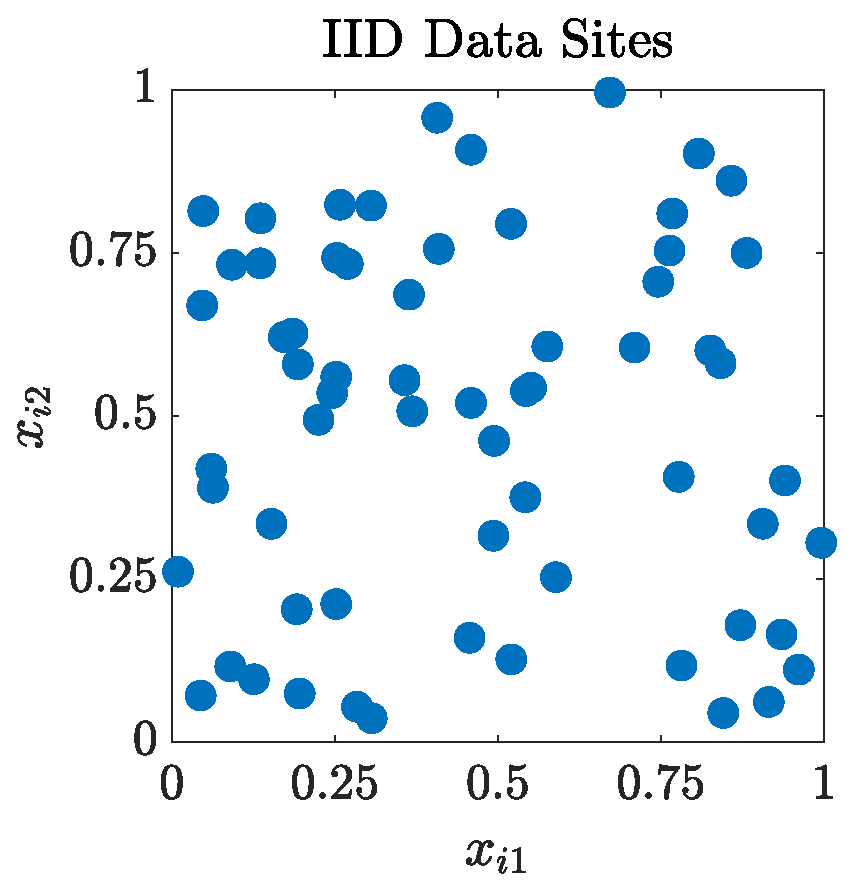
\includegraphics[width = 0.20\textwidth]{ProgramsImages/IIDPoints.eps} \ 
	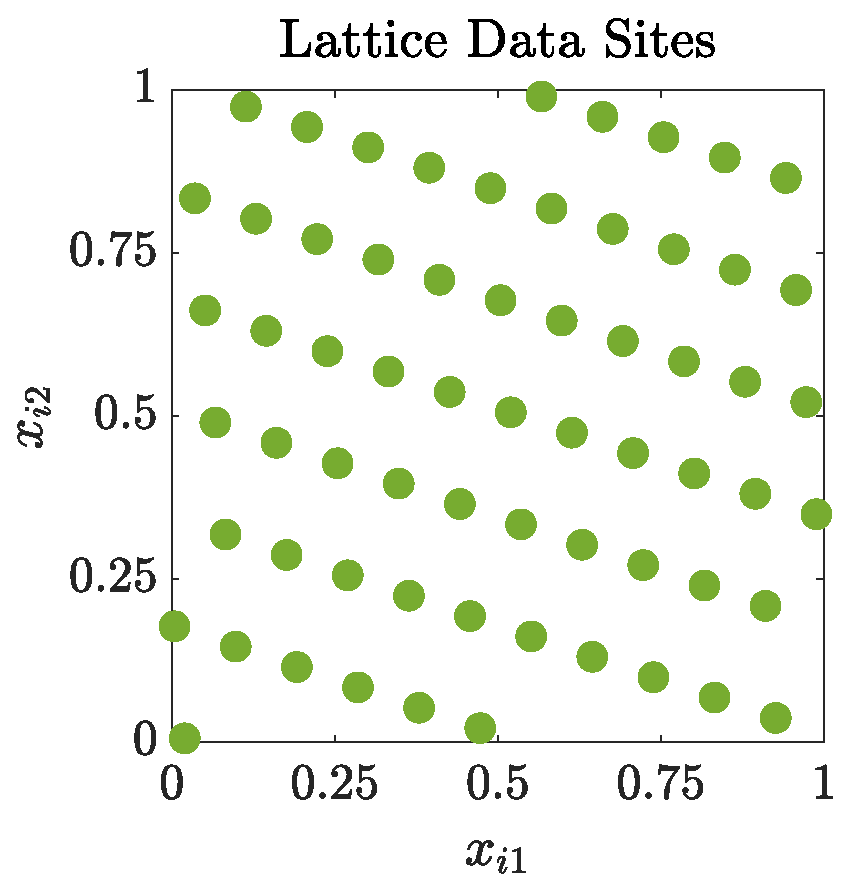
\includegraphics[width = 0.20\textwidth]{ProgramsImages/ShiftedLatticePoints.eps}  \ 
	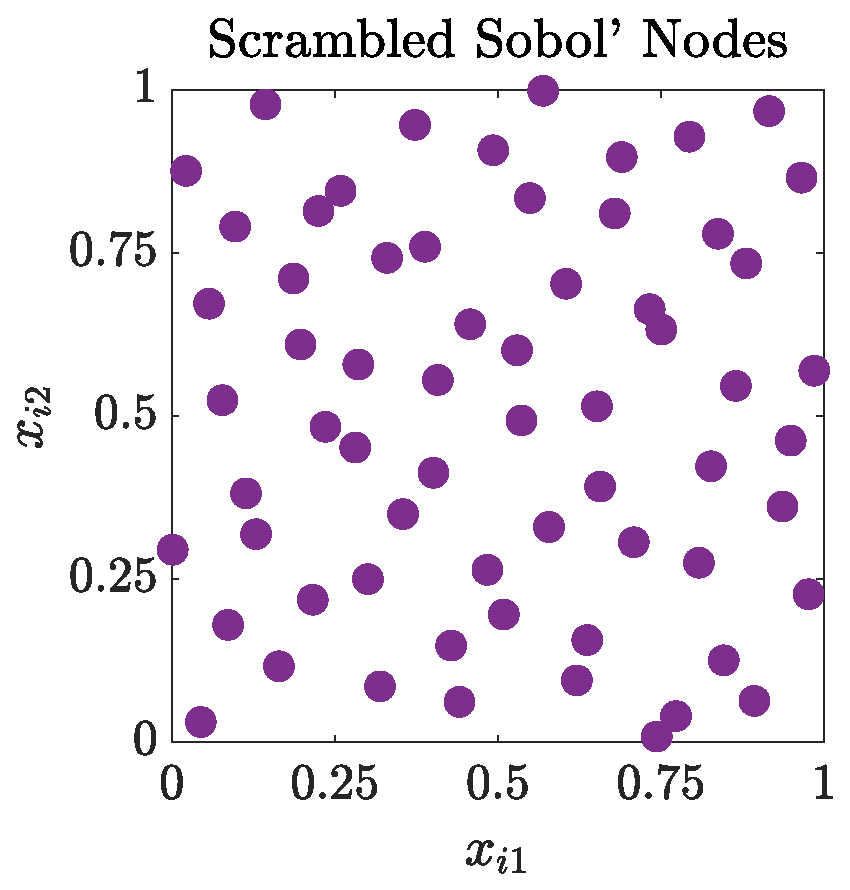
\includegraphics[width = 0.20\textwidth]{ProgramsImages/SSobolPoints.eps} 
	
	\caption{IID data sites contrasted with two families of space filling data sites.\label{PtsFig}}
\end{wrapfigure}

The goal of the initial exploratory samples is to explore the space of feasible POIs, $\Omega$,  when little, or nothing, is known about the response QOIs.  We use  Sobol' points or other low space filling data sites \cite{DicPil10a} in $\Omega$.  Fig.\ \ref{PtsFig} contrasts two families of space filling data sites with the IID data sites that cover the domain poorly. We  will compare the effectiveness of low discrepancy samples from either uniform and arcsine (Chebyshev) distributions.
The arcsine distribution pushes points towards the boundaries and is known to improve the accuracy of interpolation in one dimension.  
In higher dimensions, it may or may not help \cite{HicLi12a}.

This exploratory set of $n_0$ samples sites does not depend on $f$ or the QOIs and must be small enough to be economical, but large enough to detect important features of $f$ that influence $\QOI(f)$. The large scale simulation is run for each of these POI vectors to obtain $f(\bx_1), \ldots, f(\bx_{n_0})$, and then we begin the exploitation step.

%%%%%%%%%%%%%%%%%%%%%%%%%%%%%%%%%%%%%%%%%%%%%%%%%%%%%%%%%%%%%%%%%%%%%%%%%%%%%%%%%%%
\subsection{The Exploitation Stage:  Surrogate Model and Acquisition} \label{sec:SurrMod}
%%%%%%%%%%%%%%%%%%%%%%%%%%%%%%%%%%%%%%%%%%%%%%%%%%%%%%%%%%%%%%%%%%%%%%%%%%%%%%%%%%%

In the exploitation step, we create surrogate models, $\SURR(n,\mX,\by)$ defined on $\Omega$ by combining an MLS model to capture the mean field behavior of the response surface with a 
variation RKHS minimum norm interpolant or kriging Gaussian Process model to estimate the variation in the model. 
 
%%%%%%%%%%%%%%%%%%%%%%%%%%%%%%%%%%%%%%%%%%%%%%%%%%%%%%%%%%%%%%%%%%%%%%%%%%%%%%%%%%%
\subsubsection{The Trend Model via MLS} \label{sec:trend}
%%%%%%%%%%%%%%%%%%%%%%%%%%%%%%%%%%%%%%%%%%%%%%%%%%%%%%%%%%%%%%%%%%%%%%%%%%%%%%%%%%%
We define our trend model as the MLS approximant
\begin{equation} \label{eq:MLS}
\STREND(n,\mX,\by)(\bx) = f_{\LS}(\bx), \qquad \text{where } f_{\LS} = \argmin_{g \in \calp} \sum_{i=1}^n w_i(\bx)(y_i - g(\bx_i))^2,
\end{equation}
where $\calp$ is a finite dimensional vector space, e.g., low degree polynomials.  The weights $w_i(\bx)$ decreases with the distance $\norm[2]{\bx - \bx_i}$.   We will initially use a Gaussian kernel weight,  $w_i(\bx) = \me^{-\norm[2]{\bx - \bx_i}^2/\sigma(\bx)^2}$, where $\sigma(\bx)$ is the mean distance from the evaluation point, $\bx$, to a set of $K_n$ nearest neighbors.  The number of nearest neighbors will be greater than the dimension of $\calp$.

Every time the MLS interpolant is evaluated, we  solve a least squares systems that  weights the nearby points much more than the distant points. For the problems we are considering,
\begin{wrapfigure}{r}{0.5\textwidth}
	  \begin{center}
	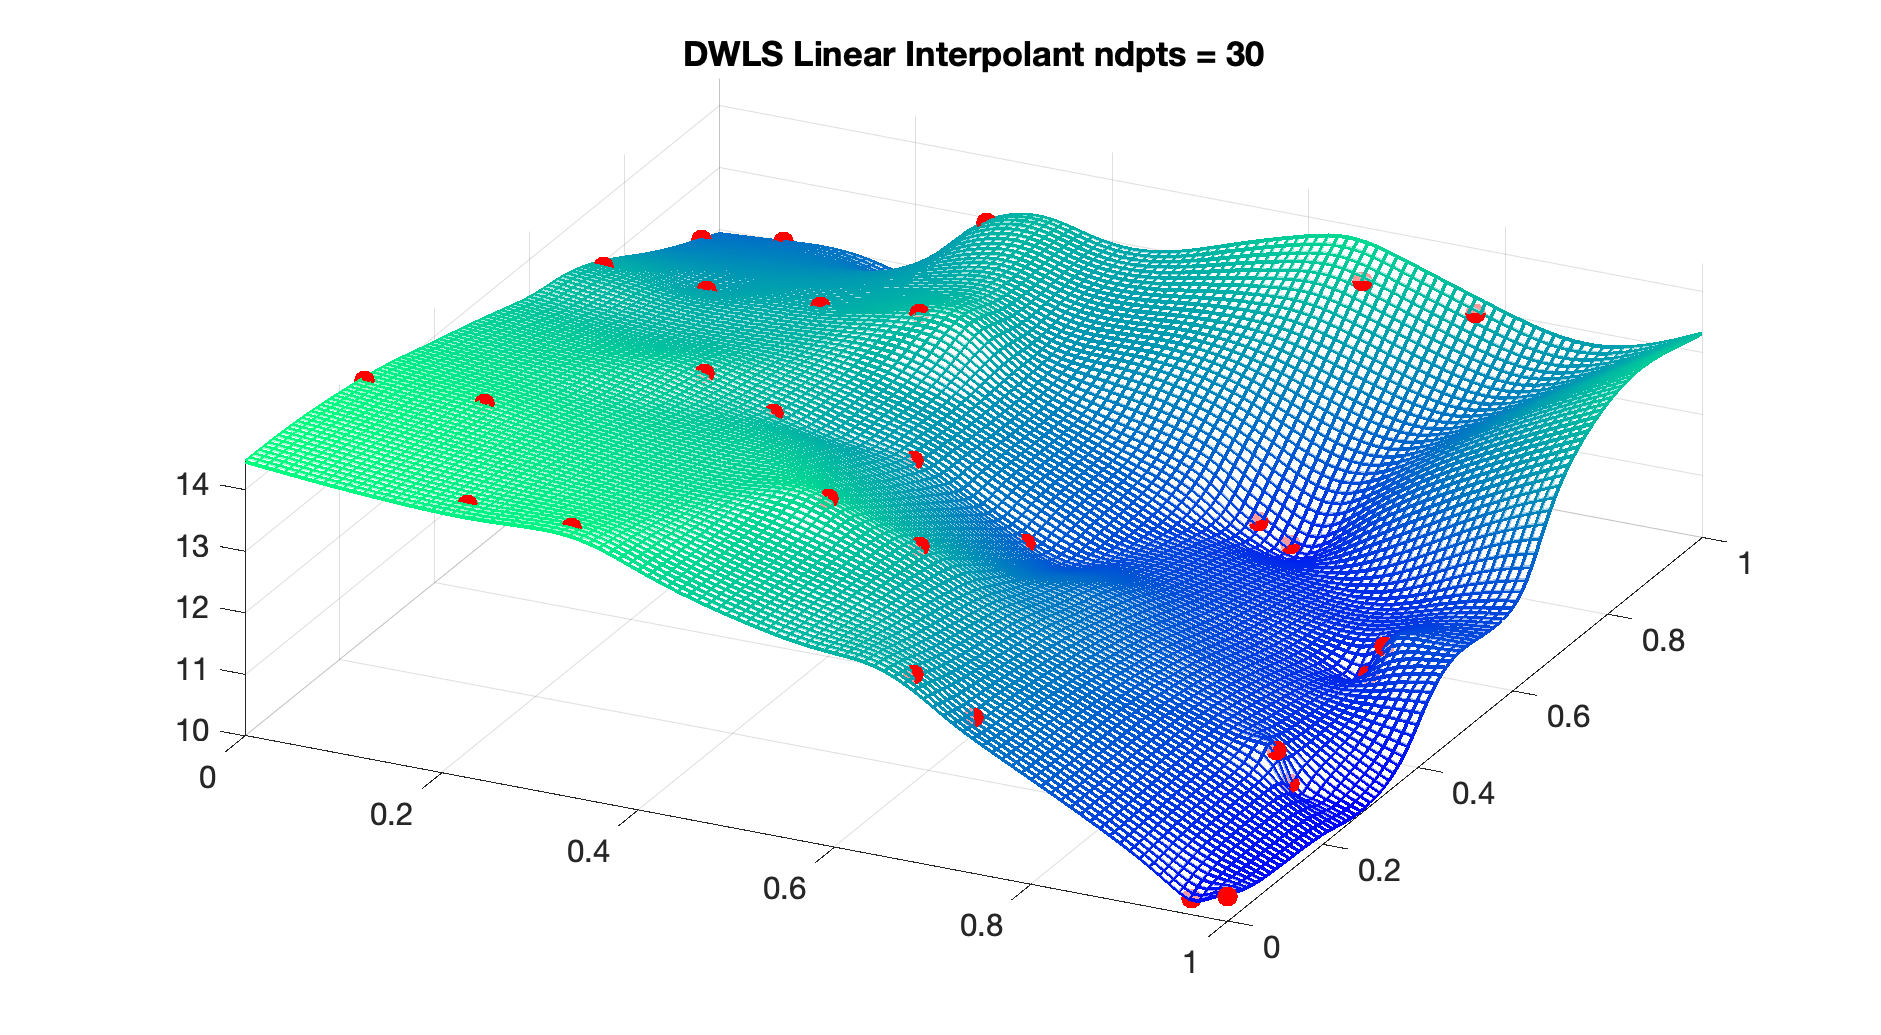
\includegraphics[width = 0.5\textwidth]{ProgramsImages/bigsurT.pdf}
	 \end{center}
	\caption{The  MLS  quasi-interpolant with linear basis functions of scattered data {$\color{red}*$} of  Big Sur sea bottom data \cite{franke1979critical}. The locally linear MLS trend model is able to fit very irregular surfaces.
	\label{MLS}}
\end{wrapfigure}
this additional computation is minimal compared to the expense of obtaining the sample values.  Note that the trend model exactly reproduces $f \in \calp$.

  
If $\calp$ consists of all polynomials of total degree up to $k$, then its dimension grows exponentially as ${k + d \choose k} $ and  will far exceed $n$ for even modest $k$ and high $d$.   We will typically choose $\calp$ to be quadratic polynomials for low dimensional problems $d<10$, and linear basis functions for high-dimensional problems.    
Polynomial approximants are very `stiff', these MLS approximnants are flexible and can fit odd surfaces similar to the way splines can approximate nonpolynomial shaped data in one dimension. 
Figure \ref{MLS} illustrates the flexibility of a  MLS with linear basis function fitting scattered data in two dimensions.  


%%%%%%%%%%%%%%%%%%%%%%%%%%%%%%%%%%%%%%%%%%%%%%%%%%%%%%%%%%%%%%%%%%%%%%%%%%%%%%%%%%%
\subsubsection{The Variation Model via RKHS/Kriging}  \label{sec:varmodel}
%%%%%%%%%%%%%%%%%%%%%%%%%%%%%%%%%%%%%%%%%%%%%%%%%%%%%%%%%%%%%%%%%%%%%%%%%%%%%%%%%%%
The trend model $\STREND(n,\mX,\by)$ is a quasi-interpolant because it does not exactly agree with the function values at each data point.  Having modeled the general trend of the output map $f$, we now model its variation, $f_{\VAR} = f - \STREND(n,\mX,\by)$ using a minimum norm RKHS interpolant.  Suppose that $f_{\VAR}$, belongs to an RKHS $\calf$.  A commonly used reproducing kernel is the following member of the Mat\'ern family:
\begin{equation} \label{eq:MatKer}
    K(\bt,\bx) = (1 + \theta \norm[2]{\bt-\bx}) \exp(-\theta\norm[2]{\bt-\bx}),
\end{equation}
where $\theta$ is a parameter to be set or inferred.  See \cite{Buh00, Fas07a, FasMcC15a, ForFly15a, ForEtal09, SchWen06a, Wen05a} for an explanation of function approximation in RKHSs.  The minimum norm interpolant of $f_{\VAR}$ in this $\calf$ using the residual data,
\begin{equation*}
    \by_{\VAR} = \by - \by_{\TREND}, \qquad \text{where }\by_{\TREND} = \bigl(\STREND(n,\mX,\by)(\bx_i) \bigr)_{i=1}^n \text{is the trend data},
\end{equation*}
is the surrogate variation model
\begin{equation} \label{appxExOne}
    \SVAR(n,\mX,\by_{\VAR}) = \sum_{i=1}^n c_i K(\cdot, \bx_i), \quad \text{where } \bc = \mK^{-1} \by_{\VAR}, \quad \mK = \mK(\mX) = \bigl( K(\bx_i,\bx_j) \bigr)_{i,j=1}^n, 
\end{equation}
which has a known pointwise error bound of
\begin{align}
\label{RKHSErrBd}
    \abs{f(\bx) - \SVAR(n,\mX,\by_{\VAR})(\bx)} & \le \sqrt{K(\bx,\bx) - \bk^T(\bx) \mK^{-1} \bk(\bx)} \, \norm[\calf]{f_{\VAR} - \SVAR(n,\mX,\by_{\VAR})} \\
    \nonumber
    & \le \sqrt{K(\bx,\bx) - \bk^T(\bx) \mK^{-1} \bk(\bx)} \, \norm[\calf]{f_{\VAR}} \qquad \forall f_{\VAR} \in \calf, \ \bx \in \Omega \\
    \nonumber
    & \qquad \qquad \text{where }  \bk(\bx) = \bigl(K(\bx,\bx_i) \bigr)_{i=1}^n.
\end{align}

To make the error bound for the surrogate model data driven, let $\calc$ be the cone of functions whose norms are approximated modestly well by the norms of their surrogates:  
\begin{align}  \label{RKHScone}
    \calc &:= \Bigl\{f_{\VAR} \in \calf : \norm[\calf]{f_{\VAR} - \SVAR(n,\mX,\by_{\VAR})} \le A_n \bignorm[\calf]{\SVAR(n,\mX,\by_{\VAR})} \Bigr \} \\
    \nonumber
    & = \Bigl\{f_{\VAR} \in \calf : \norm[\calf]{f_{\VAR}}^2 \le (1 + A_n^2) \bignorm[\calf]{\SVAR(n,\mX,\by)}^2 \Bigr \},
\end{align}
where $A_n$ is positive, and fixed in advance.  This $\calc$ is a cone because if $f_{\VAR} \in \calc$, then $c f_{\VAR} \in \calc$ for any real $c$.  The intuition in defining this cone is: \emph{what you have not seen is not much worse than what you can see}. All adaptive algorithms are based on this philosophy.  The definition of the cone in \eqref{RKHScone} is a way of formalizing this key idea. Noting that $\bignorm[\calf]{\SVAR(n,\mX,\by_{\VAR})} = \sqrt{\by_{\VAR} \mK^{-1} \by_{\VAR}}$ error bound \eqref{RKHSErrBd} then implies an error bound that can be computed solely based on the output data: 
\begin{subequations} \label{eq:DataErrBd}
\begin{gather}
    \abs{f_{\VAR}(\bx) - \SVAR(n,\mX,\by_{\VAR})(\bx)} \le \SVARERR(n,\mX,\by_{\VAR})(\bx) \qquad \forall f \in \calc, \\
        \label{eq:DataErrBda} 
   \text{where } \SVARERR(n,\mX,\by_{\VAR})(\bx) : = A_n \sqrt{[K(\bx,\bx) - \bk^T(\bx) \mK^{-1} \bk(\bx)] \, [\by_{\VAR}^T \mK^{-1} \by_{\VAR}] }.
\end{gather}
\end{subequations}
This data-driven error bound for the surrogate variation model is used to construct the  acquisition functions in \eqref{eq:QOIval} and error bounds in \eqref{eq:QOIerr} for the two QOIs in \eqref{eq:ourQOIs} with their approximations in \eqref{eq:QOIhat}.

One may question why the surrogate error bound in \eqref{eq:DataErrBd} only applies to some subset, $\calc$, of the space, $\calf$, of possible functions, $f_{\VAR}$.  Since $\calf$ is infinite dimensional, no matter what $n$ output data are observed, there is always some $f_\perp \in\calf$ that is zero at every data site.  The surrogate variation models for $f_{\VAR} \pm c f_\perp$, must be the same for all $c$, while the values of $f_{\VAR} + c f_\perp$ and  $f_{\VAR} - c f_\perp$ can be made arbitrarily far apart for large enough $c$.  Thus, the same surrogate variation error bound cannot apply for all possible $f_{\VAR} + c f_\perp$.

The deterministic framework using RKHSs for $f_{\VAR}$ has a parallel Bayesian interpretation or probabilistic numerics promoted by Diaconis \cite{Dia88a} and pursued by many others \cite{BriEtal18a, OHa91a, OwhEtal19a, RasWil06a, Rit00a}.  It assumes that $f_{\VAR}$ is an instance of $\GP(0,K)$, a Gaussian process with mean zero and covariance kernel, $K$.  In this case the posterior mean of $f_{\VAR}(x)$ given the data $(\mX,\by)$ is called a kriging model and has the same expression as $\SVAR(n,\mX,\by)$ as in \eqref{appxExOne}, and width of the pointwise credible interval for the surrogate variation model is the same as $\SVARERR(n,\mX,\by)$ in \eqref{eq:DataErrBd}, with $A_{10} \approx 1$ determined by empirical Bayes.  In this research we will adopt the deterministic and/or Bayesian approach, depending on which better suits our needs.

There are some weaknesses with the common RKHS/kriging approach.  The reproducing/covariance kernels, $K$, typically used do not sufficiently adapt to the observed function data.  We will address this is in Sect.\ \ref{sec:kerinferdata}.  Also, for large $d$, a kernel based on Euclidean distance, as is the case in \eqref{eq:MatKer}, may be victim to the curse of dimensionality.  We will address this is in Sect.\ \ref{sec:selectCoord}.


%%%%%%%%%%%%%%%%%%%%%%%%%%%%%%%%%%%%%%%%%%%%%%%%%%%%%%%%%%%%%%%%%%%%%%%%%%%%%%%%%%%
\subsubsection{Bayesian Bootstrapping to Determine Surrogate Model Uncertainty} \label{sec:BayesianBootUncertainty}
%%%%%%%%%%%%%%%%%%%%%%%%%%%%%%%%%%%%%%%%%%%%%%%%%%%%%%%%%%%%%%%%%%%%%%%%%%%%%%%%%%%
The uncertainty in our surrogate variation models, $\SVARERR(n,\mX,\by)$, could serve as our surrogate model uncertainty.  However, given the small number of data used to construct our models and the relatively large number of POIs involved, we propose to overlay another measure of uncertainty on top for the sake of robustness.  

In classical bootstrapping, a new sets of samples are generated by randomly selecting the existing samples, with replacement.  
In small sample situations, removing even a few samples from the least squares fit can create  large variations in the trend model. In the weighted Bayesian bootstrap algorithm, all of the samples are used for each trend model and each sample $x_i$ is randomly weighted by the factor $w_i \in [0,1]$. By using all the samples, the weighted Bayesian bootstrap method provides a more robust estimate for uncertainty quantification in small samples than the classical bootstrap method  \cite{rubin1981bayesian, efron1986bootstrap, efron2016computer}.    

In our weighted Bayesian bootstrap algorithm, we generate an ensemble of $B$ trend models by extending \eqref{eq:MLS}
\begin{equation}
    \STREND^b(n,\mX,\by)(\bx) = f^b_{\LS}(\bx), \qquad \text{where } f^b_{\LS} = \argmin_{g \in \calp} \sum_{i=1}^n v_i^b w_i(\bx)(y_i - g(\bx_i))^2,
\end{equation}
where as in Sect.\ \ref{sec:trend}, the $w_i$ are the MLS weight functionss, and now $\bv^b$ is an $n$-vector uniformly distributed over the unit simplex, $\cals^n : = \{\bv \in [0,1]^n : v_1 + \cdots + v_n = 1\}$.  We then define the bootstrap residuals at the data points $\by^b_{\TREND} = f^b_{\LS}(\bx)$. 

For each trend model, $\STREND^b(n,\mX,\by)$, we construct the an associated variation model, $\SVAR^b(n,\mX,\by - \by^b_{\TREND})$ and its uncertainty, $\SVARERR^b(n,\mX,\by - \by^b_{\TREND})$.  These lead to our final surrogate model and its uncertainty.
The surrogate model for each Bayesian bootstrap model can be expressed as 
\begin{equation*}
    \SURR^b(n,\mX,\by) = \STREND^b(n,\mX,\by) + \SVAR^b(n,\mX,\by - \by^b_{\TREND}).
\end{equation*}
These can be averaged to define the mean surrogate model
\begin{equation} \label{eq:SMBoot}
    \SURR(n,\mX,\by) = \frac 1B \sum_{b=1}^B \SURR^b(n,\mX,\by), 
\end{equation}
and the  surrogate uncertainty model is defined by the \FJHNote{Not sure in which sense this is unbiased} unbiased estimate
\begin{equation} \label{eq:SUBoot}
    \SURRERR(n,\mX,\by) = \sqrt{\frac{1}{B-1} \sum_{b=1}^B \Bigl\{ \bigl[ \SURR^b(n,\mX,\by) - \SURR(n,\mX,\by) \bigr]^2 + [\SVARERR^b(n,\mX,\by)]^2 \Bigr\} } .
\end{equation}
We are not certain if this simple estimate is the best measure of uncertainty.  We will explore alternatives to identify if there are better approaches to combine the ensemble of uncertainty estimates.

%%%%%%%%%%%%%%%%%%%%%%%%%%%%%%%%%%%%%%%%%%%%%%%%%%%%%%%%%%%%%%%%%%%%%%%%%%%%%%%%%%%
\subsubsection{Acquisition via the Surrogate Model} \label{sec:acquire}
%%%%%%%%%%%%%%%%%%%%%%%%%%%%%%%%%%%%%%%%%%%%%%%%%%%%%%%%%%%%%%%%%%%%%%%%%%%%%%%%%%%

Given the surrogate model in \eqref{eq:SMBoot} and its uncertainty in \ref{eq:SUBoot}, we may then define the acquisition functions for function and approximation respectively:
\begin{subequations} \label{eq:QOIval}
\begin{align}
\label{eq:idval}
     \IDVAL(\bx,n,\mX,\by) &= \SURRERR(n,\mX,\by)(\bx), \\
     \label{eq:minval}
      \MINVAL(\bx,n,\mX,\by) &= \APPMIN(n,\mX,\by) - [f(\bx) - \SURRERR(n,\mX,\by)(\bx)].
\end{align}
\end{subequations}
The next data site, $\bx_{n+1}$ maximizes the acquisition function (see \eqref{eq:nextsample}).  For function approximation we sample next where the surrogate model uncertainty is greatest.  For optimization we sample next where the output might be smallest.

To maximize the acquisition functions, we first evaluate them on a candidate set, $\mX^c := (\bx^c_1, \ldots, \bx^c_n)^T$, where $n_c \gg n$.  Once near maximizers have been identified, then further maximization can be obtained wither by searching nearby or switching to a numerical optimization algorithm.  We will consider both of these approaches. 

The acquisition functions are also related to the error bounds that we expect to derive for our algorithms:
\begin{subequations} \label{eq:QOIerr}
\begin{align}
\label{eq:iderr}
     \bignorm[\infty]{f - \APPID(n,\mX,\by)} &\le \norm[\infty]{\SURRERR(n,\mX,\by)} =: \IDERR(n,\mX,\by), \\
     \label{eq:minerr}
     \bigabs{\MIN(f) - \APPMIN(n,\mX,\by)} & \le \max_{\bx \in \Omega} \Bigl\{ \APPMIN(n,\mX,\by) - [f(\bx)- \SURRERR(n,\mX,\by)](\bx) \Bigr\} \\
     \nonumber
     & =: \MINERR(n,\mX,\by).
\end{align}
\end{subequations}
These error bounds should be valid for $\calc$,  precisely defined sets of well-behaved simulation output maps, $f$.  The identification of these $\calc$ is part of our research.  Hints appear in Sect.\ \ref{sec:varmodel}. 


%%%%%%%%%%%%%%%%%%%%%%%%%%%%%%%%%%%%%%%%%%%%%%%%%%%%%%%%%%%%%%%%%%%%%%%%%%%%%%%%%%%
\section{Intellectual Merit of the Proposed Research} \label{sec:Proposed}
%%%%%%%%%%%%%%%%%%%%%%%%%%%%%%%%%%%%%%%%%%%%%%%%%%%%%%%%%%%%%%%%%%%%%%%%%%%%%%%%%%%

%%%%%%%%%%%%%%%%%%%%%%%%%%%%%%%%%%%%%%%%%%%%%%%%%%%%%%%%%%%%%%%%%%%%%%%%%%%%%%%%%%%%
\subsection{Existing Adaptive Sampling Schemes and Their Shortcomings} \label{sec:shortExist}
%%%%%%%%%%%%%%%%%%%%%%%%%%%%%%%%%%%%%%%%%%%%%%%%%%%%%%%%%%%%%%%%%%%%%%%%%%%%%%%%%%%

We summarize the existing literature on adaptive sampling \cite{aute2013cross,burnaev2015adaptive,fu2017adaptive,gramacy2008adaptive,jin2002sequential,kleijnen2004application}. A number of popular adaptive design criteria are constructed based on an acquisition function, that does not depend on the simulation output data, but only on the data sites, i.e., $\VAL(n,\mX,\by) = \VAL(n,\mX)$.  Such adaptive designs fill in wholes in the existing design according to a particular criteria, including those below. 
\begin{description}
    \item[Discrepancy] This measures the difference between the empirical distribution of the design and the target (usually uniform) distribution \cite{FangEtal19a}.  Examples of low discrepancy designs are given in Fig.\ \ref{PtsFig}.  
    \item[Covering radius or fill distance] This is the minimum radius needed for balls centered at each data site to cover the whole domain, $\Omega$.  Minimax designs minimize this criterion.
    \item[Minimium distance between data sites]  Maximin designs maximize this criterion \cite{jin2002sequential}.
    \item[Entropy] Designs maximizing entropy seek to maximize the information when choosing the next data site \cite{jin2002sequential}.  They also typically assume a known Gaussian process model.
\end{description}
Orthogonal arrays and Latin hypercube sampling are further examples of space filling designs, although they are not usually constructed sequentially.  We will use space filling designs are useful for our exploration stage, but they are inadequate for the exploitation stage of our adaptive algorithms because they do not include the output data in a meaningful way.  

Some existing adaptive sampling methods use a jackknife and leave-one-out cross-validation adaptive sampling to measure the variation in predictions based on leaving out one observation at a time \cite{aute2013cross,jin2002sequential, kleijnen2004application}.  However, these approaches often tend to pick the next data site close to an existing one \cite{jin2002sequential}, which is wasteful.  A fix has been proposed to include a penalty that discourages choosing the next data site close to an existing one \cite{aute2013cross,jin2002sequential}.

%%%%%%%%%%%%%%%%%%%%%%%%%%%%%%%%%%%%%%%%%%%%%%%%%%%%%%%%%%%%%%%%%%%%%%%%%%%%%%%%%%%
\subsection{Surrogate Trend Models} \label{sec:ourtrend}
%%%%%%%%%%%%%%%%%%%%%%%%%%%%%%%%%%%%%%%%%%%%%%%%%%%%%%%%%%%%%%%%%%%%%%%%%%%%%%%%%%%
Global parametric surrogate models can capture the trend of a multivariate response surface only if the data is fit well by the parametric model over all the domain.  For example, in one-dimensional problems low-degree polynomials can capture simple trends in the data, but fail to accurately represent nonpolynomial shapes, such as Gaussians  or step functions.  Piecewise polynomial interpolants, such as cubic Hermite polynomials, can effectively represent these surfaces, but don't generalize easily to very high dimensions with scattered  data.  

The MLS quasi-interpolants are an effective alternative to piecewise polynomials in that they use a moving fit of local low-degree polynomials to capture global nonpolynomial behavior.  The additional computational cost to solve for the coefficients whenever they are evaluated is small compared to the cost of generating new samples.  

One of the challenges in MLS is to identify a robust methodology for picking the appropriate  length scale, $\sigma(\bx)$, for the MLS kernel.  Our current approach is to define this length scale as the mean distance to the nearest $K_n$ neighbors of $\bx$, where $K_n$ is greater than the number of basis functions, $K_p$  in the local approximating function is based on empirical experiments.  
This heuristic approach usually identifies a good balance between the relative weights of the nearby and distant points so that the Moore Penrose matrix for the least squares problem is well conditioned.  If the least squares problem is ill-conditioned, then the length scale is increased.  We propose to analyze this heuristic approach and identify a procedure, along the lines of the adaptive Armijo rule in numerical optimization \cite{kelley1999iterative} to select the local length scale based on a more mathematical foundation.

Another shortcoming of the existing MLS quasi-interpolants is that they treat every coordinate direction the same.  
\emph{We will extend the MLS to use the full covariance matrix in the multivariate Gaussian kernel based on the relative variation in underlying active dimensional analysis}. We will  describe some of these ideas in section \ref{sec:selectCoord}.  

%%%%%%%%%%%%%%%%%%%%%%%%%%%%%%%%%%%%%%%%%%%%%%%%%%%%%%%%%%%%%%%%%%%%%%%%%%%%%%%%%%%
\subsection{Data-Based Inferred Kernels for Surrogate Variation Models} \label{sec:kerinferdata}
%%%%%%%%%%%%%%%%%%%%%%%%%%%%%%%%%%%%%%%%%%%%%%%%%%%%%%%%%%%%%%%%%%%%%%%%%%%%%%%%%%%

To illustrate some of the weaknesses of the typical RKHS/kriging approach in Sect.\ \ref{sec:varmodel} we consider the following univariate function, which has a mean value near zero:
\begin{equation} \label{eq:univarfun}
f_{\VAR} \colon x \mapsto \exp(-6x) \sin(8x+0.1) - 0.1.
\end{equation}
This $f_{\VAR}$ is displayed in Fig.\ \ref{fig:sampleFun} along with its surrogate model $\SVAR(10,\mX,\by)$ based on the $n=10$ point design $\mX = (0, 0.1, \ldots, 0.6, 0.8, 0.9, 1)^T$ and the Mat\'ern kernel in \eqref{eq:MatKer} with $\theta =1$.  
Although not highly accurate, $\SURR(10,\mX,\by)$ captures the peak on the left because the data sites are dense enough there.  If the design consists only of the $n=4$ sparse data sites, $\mX = (0, 0.4,  0.6, 1)^T$, then $\SURR(4,\mX,\by)$ misses the peak, as shown in Fig.\ \ref{fig:sampleFun}. This demonstrates the need for the sufficient samples in the explore stage highlighted in Sect.\ \ref{sec:Explore}. 

\begin{figure}[ht]
    \centering
    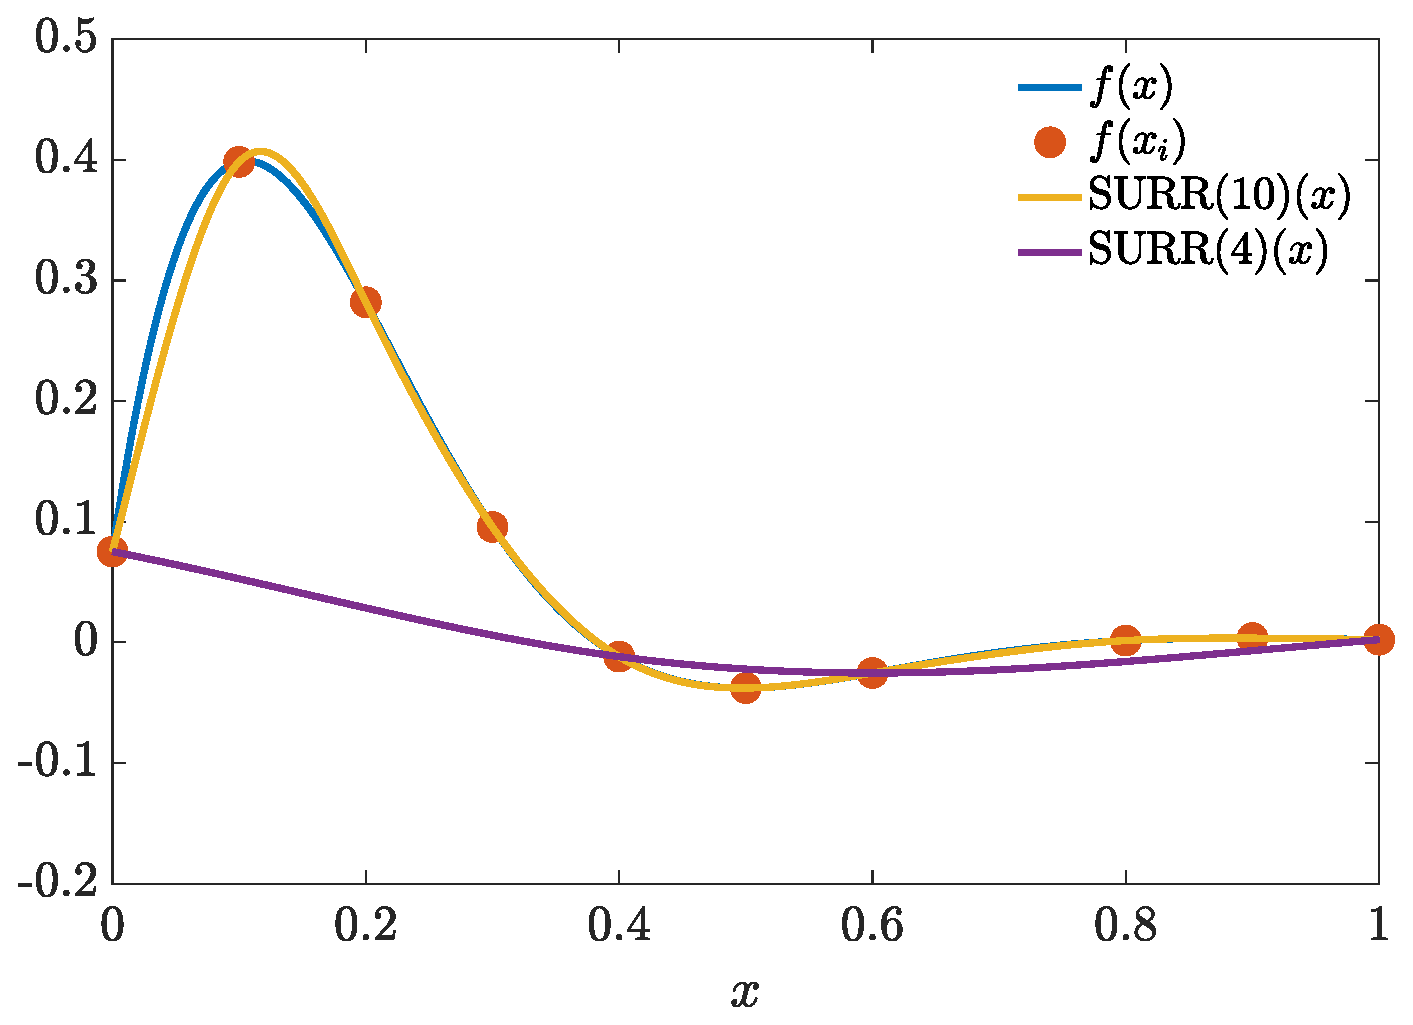
\includegraphics[width = 7cm]{ProgramsImages/fandDataAndAppxSmall.eps} \qquad \qquad
    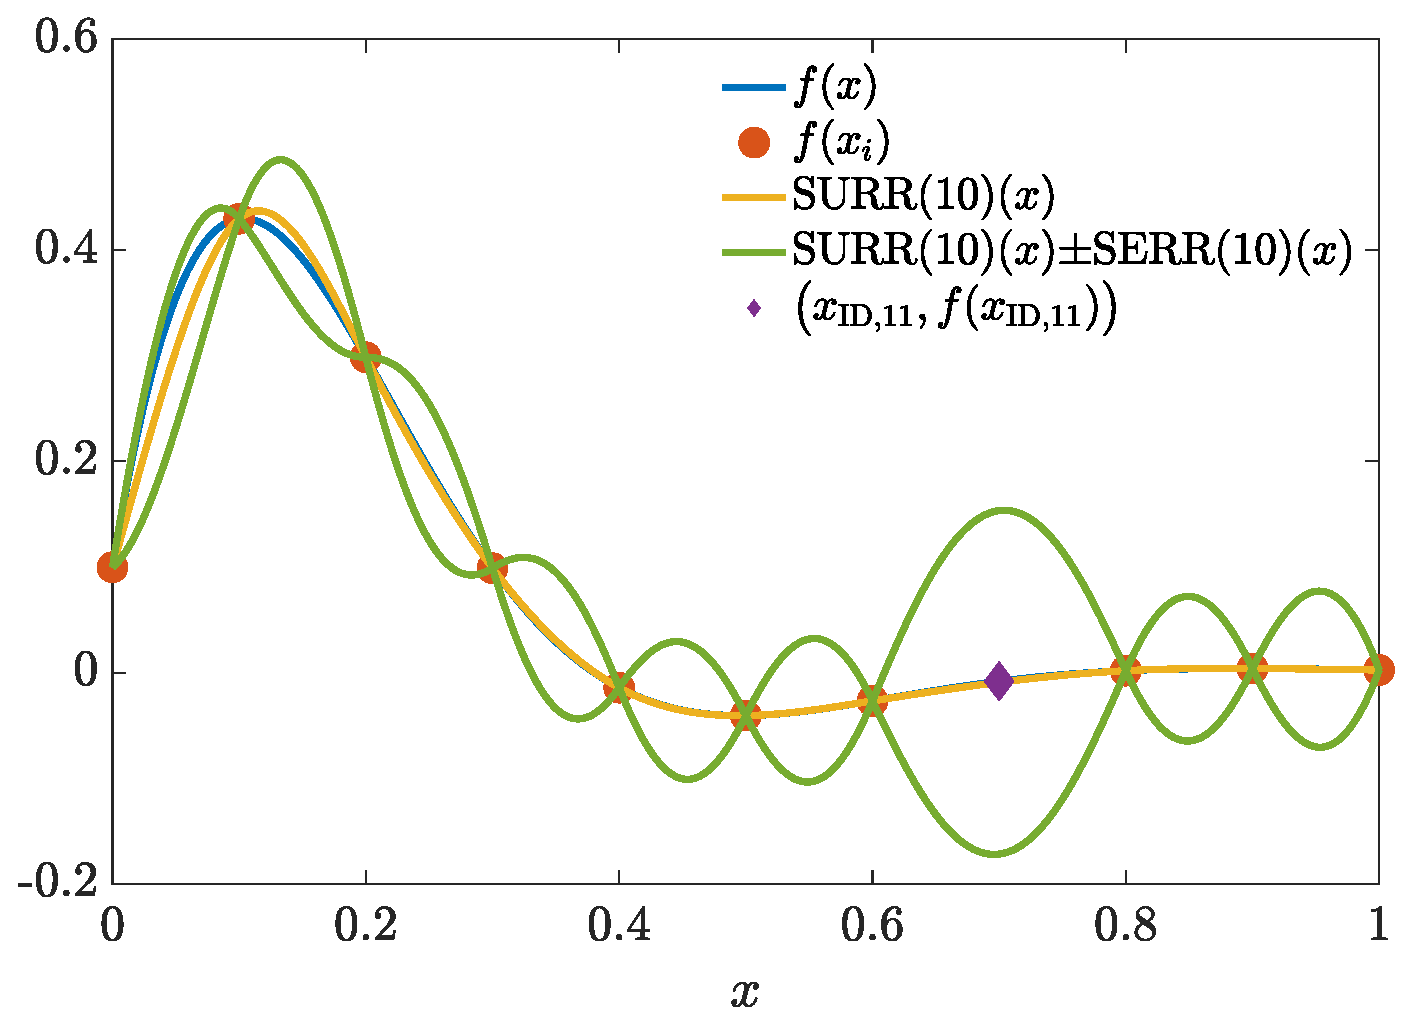
\includegraphics[width = 7cm]{ProgramsImages/fandDataAndAppxAndRMSPE.eps}
    \caption{The left plot shows $f_V$ in \eqref{eq:univarfun} and its surrogate variation model \eqref{appxExOne} using $10$ and $4$ data sites and the kernel \eqref{eq:MatKer} with $\theta = 1$. Too few date sites yields a poor approximation.  The right plot includes the surrogate variation uncertainty, $\SVARERR(10,\mX,\by)$ from \eqref{eq:DataErrBda} with $A_{10} =1$, and the location of the largest uncertainty, $x_{11}$. The largest true error occurs far away from $x_{11}$.}
    \label{fig:sampleFun}
\end{figure}

\iffalse
There is a substantial literature on $d$-dimensional space filling designs \cite{FangEtal19a, Jos16a, SanWilNot03}. The number of data sites required for the initial design depends on i) how many one can afford, ii) how narrow a peak one is willing to miss, and iii) the number of independent variables, $d$.
\fi

For function approximation we should choose the next data site to have where the uncertainty in $f_{\VAR}$ is largest, which would be $x_{11} = \argmax_x \SVARERR(10,\mX,\by)(x)$ as depicted in Fig.\ \ref{fig:sampleFun}.  However, $f_{\VAR}(x_{11}) \approx \SVAR(11,\mX,\by)(x_{11})$, so sampling at $x_{11}$ does not help much.

The surrogate variance model and its uncertainty are not satisfactory for several reasons: i) The form of the kernel, $K$, is not influenced by the output data, $\by$, ii) the pointwise surrogate error bound in \eqref{eq:DataErrBd} depends weakly on the output data $\by$, and consequently, iii) the surrogate variation uncertainty is tight on the left, but quite loose on the right. 

One improvement is to infer the value of $\theta$ inherent in the definition of $K$ in \eqref{eq:MatKer} rather than to set it arbitrarily. The empirical Bayes perspective leads to the following choice \cite{Hic17a}: 
\begin{equation} \label{eq:thetEB}
    \theta_{\textup{EB}} = \argmin_\theta \left[\frac 1n \log \bigl( \det(\mK_\theta) \bigr) + \log \bigl ( \by^T \mK_\theta^{-1} \by \bigr)\right].
\end{equation}
For the example $f_{\VAR}$ in \eqref{eq:univarfun}, $\theta_{\textup{EB}} = 11$, and the resulting approximation and approximate error bound are given on the left of Fig.\ \ref{fig:InferKernel}.  Unfortunately, this new surrogate model has similar deficiencies as the original one, and the suggested next data site is at a place where the function approximation is already quite good.

\begin{figure}[ht]
    \centering
    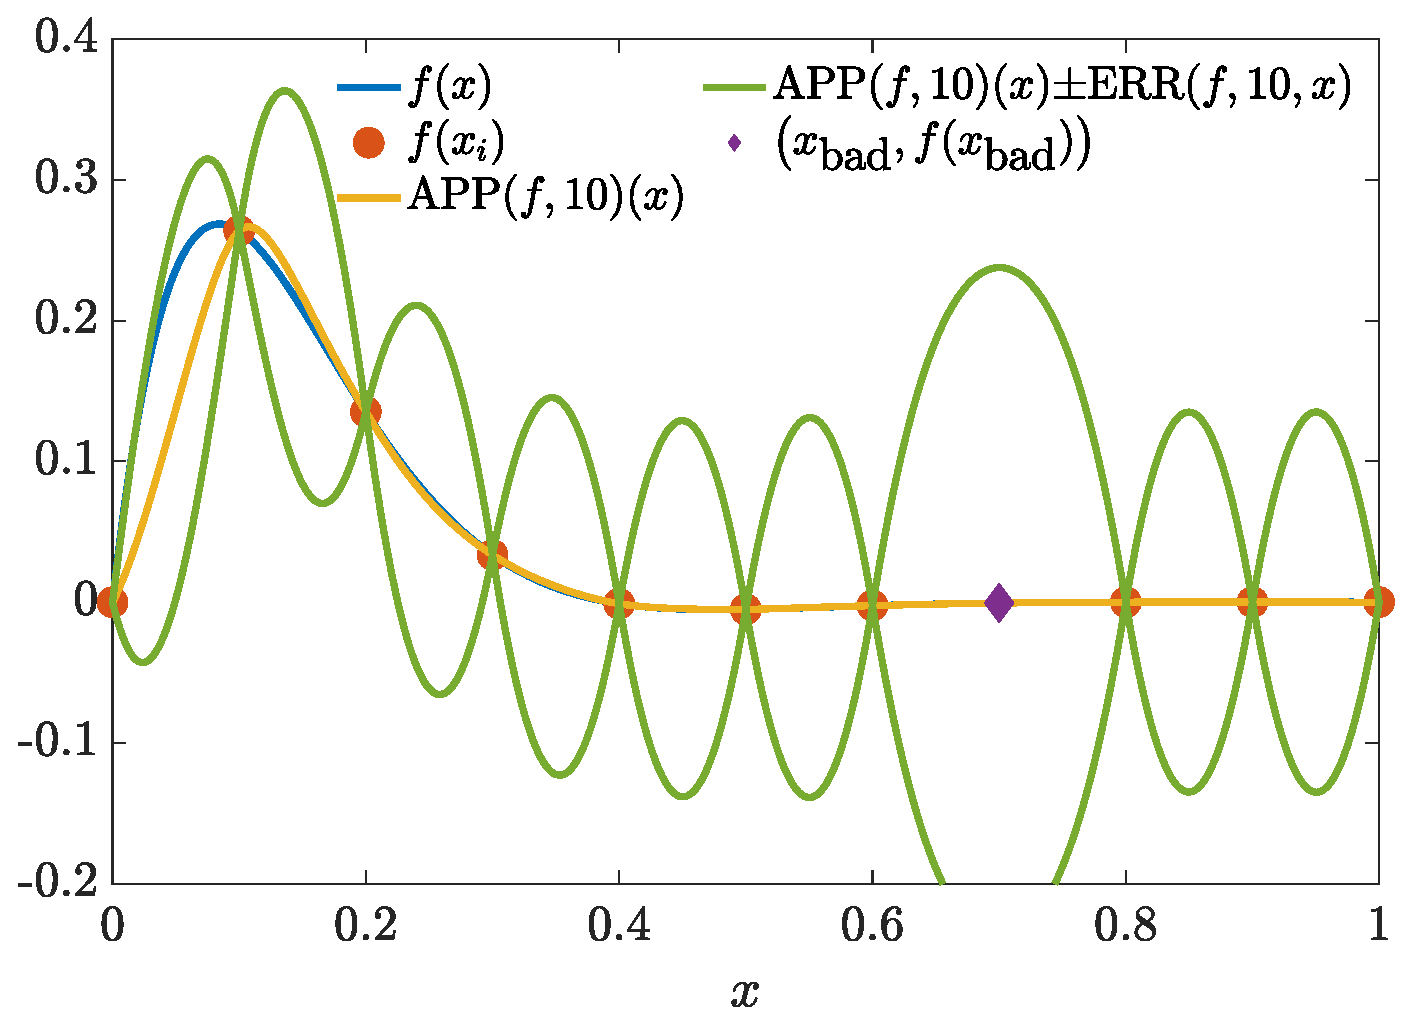
\includegraphics[width = 7cm]{ProgramsImages/fandDataAndAppxAndRMSPEOpt.eps} \qquad \qquad
    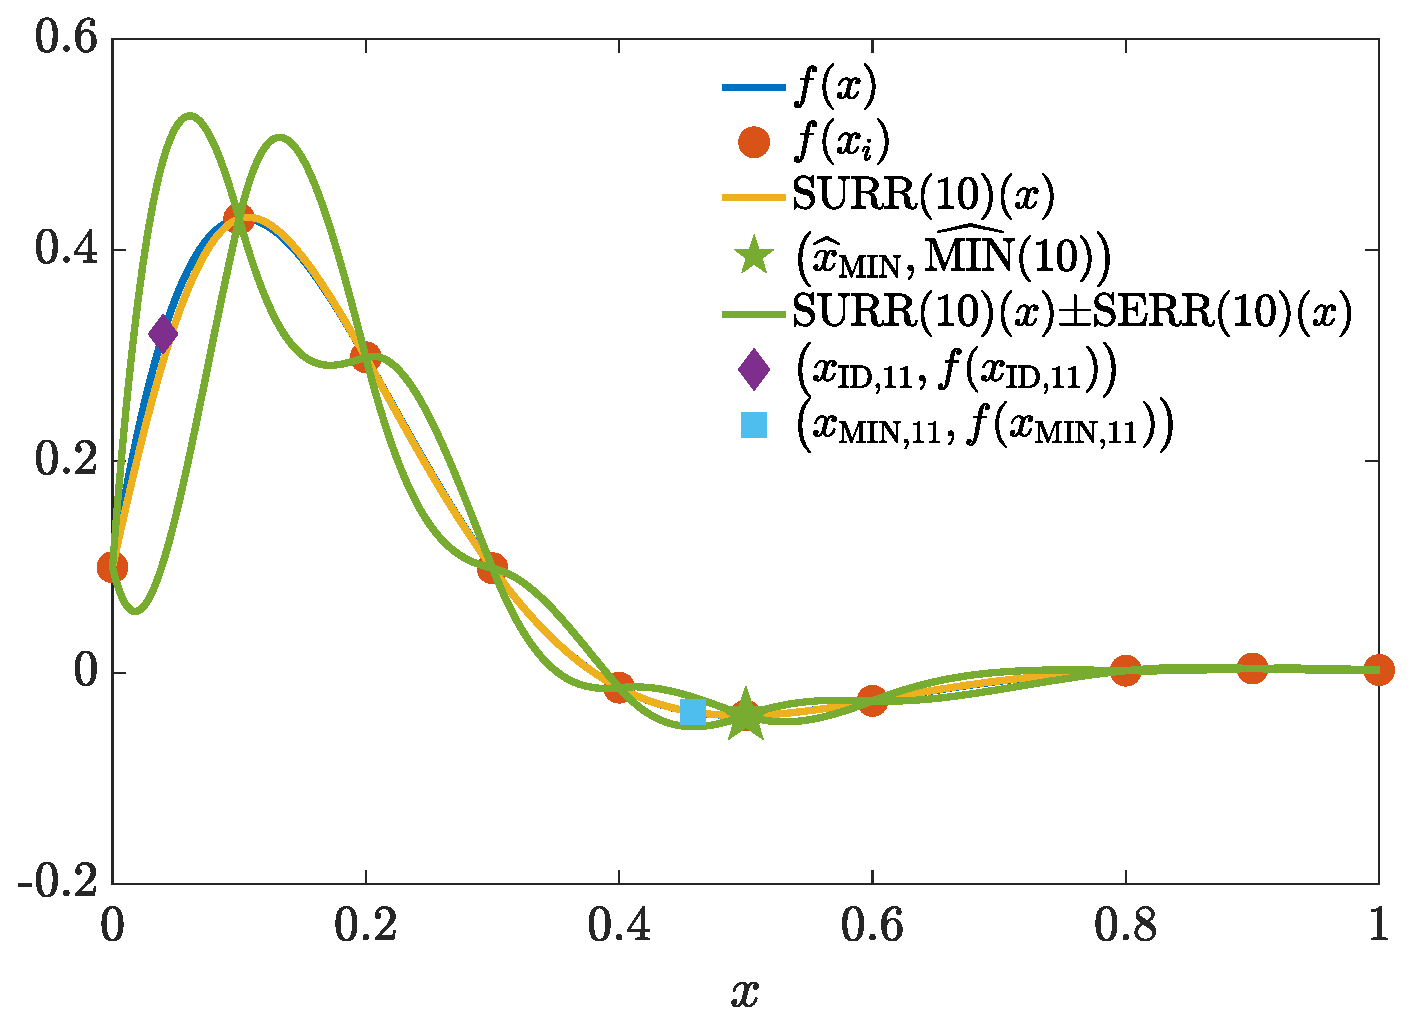
\includegraphics[width = 7cm]{ProgramsImages/fandDataAndAppxAndRMSPEOpty.eps}
    \caption{The left plot shows the surrogate variation model with its uncertainty for the example $f_{\VAR}$ in \eqref{eq:univarfun} but with $\theta = \theta_{\textup{EB}} = 11$ rather than $\theta =1$.  The approximation is slightly better than in Fig.\ \ref{fig:sampleFun}, but the uncertainty is much larger.  The right plot shows the the surrogate variation model with its uncertainty now for the modified Mat\`ern kernel in \eqref{modMatKer}, and now with $\theta = \theta_{\textup{EB}} = 5.3$ and $S = S_{\textup{EB}} = -6.0$.  The surrogate variation model is much improved, especially for smaller $x$, and the uncertainty is much smaller.  The next data site is in a location that makes intuitive sense.}
    \label{fig:InferKernel}
\end{figure}

A more helpful approach is to generalize the Mat\'ern kernel as follows to allow for the variation of the functions to be greater in one part of the domain than the other:
\begin{equation} \label{modMatKer}
    K(t,x) = \exp(S(t+x))(1 + \theta \abs{t-x}) \exp(-\theta\abs{t-x}).
\end{equation}
Here we have considered the case $d=1$.  This new kernel maintains its properties of being symmetric and positive definite because all we have done is to multiply the original kernel by $g(t)g(x)$ for some function $g$.  Here $S$ is a parameter to be inferred.

The right plot in Fig.\ \ref{fig:InferKernel} shows the surrogate variation model and its uncertainty for the example in \eqref{eq:univarfun}, but for this modified Mat\'ern kernel in \eqref{modMatKer}, with both parameters $\theta$ and $S$ being determined by empirical Bayes as in \eqref{eq:thetEB}.  Now, $\SVAR(10,\mX,\by)$ fits $f_{\VAR}$ much better and the uncertainty fits better.  The next data site, $x_{11} = \argmax_x \SVARERR(10,\mX,\by)(x)$, is in a region where $f_{\VAR}$ varies greatly. 

This example of modifying a well-known kernel so that data-based inference of the parameters produce a better approximation and a better adaptive sampling scheme is proof of concept. \emph{ We plan to extend this idea to a more general multivariate setting.}  Some of the challenges will be to ensure that our modified kernels are not over-parameterized and specifying a mathematically precise set of functions for which this approach is successful.

Another area weakness in the adaptive scheme outlined above is that the cone $\calc$ of reasonable functions defined in  \eqref{RKHScone} depends strongly on the specific design chosen, $\mX$.  We will \emph{modify the definition of $\calc$ to depend only some modest quality measure of the design}, such as the $\bx_i$ filling  $\Omega$ relatively well.  This is also a question for research.

%%%%%%%%%%%%%%%%%%%%%%%%%%%%%%%%%%%%%%%%%%%%%%%%%%%%%%%%%%%%%%%%%%%%%%%%%%%%%%%%%%%
\subsection{Selecting Important Coordinate Directions to Avoid the Curse of Dimensionality} \label{sec:selectCoord}
%%%%%%%%%%%%%%%%%%%%%%%%%%%%%%%%%%%%%%%%%%%%%%%%%%%%%%%%%%%%%%%%%%%%%%%%%%%%%%%%%%%

Approximating optimizing a $d$-variate function, $f$, using $n$ output data, where $d$ is in the dozens, and $n$ is restricted to the thousands is infeasible if $f$ is fully $d$ dimensional.  For example, even a multilinear function,
\begin{equation*}
f(\bx) = a_0 + a_1 x_1 + a_2 x_2 + \cdots + a_{1,2} x_1 x_2 + \cdots + a_{1,\ldots, d}x_1 \cdots x_d, \qquad \bx \in [-1,1]^d,
\end{equation*}
requires at least $n = 2^d$ samples to approximate or optimize well.  Exponential growth in the sample size required for a reasonable solution is called the \emph{curse of dimensionality}.  There are several ways to overcome this curse, all of which involve restricting oneself to a $\calc$ of reasonable functions that have an essentially low-dimensional structure.  We highlight a couple of ways that we will explore.

%%%%%%%%%%%%%%%%%%%%%%%%%%%%%%%%%%%%%%%%%%%%%%%%%%%%%%%%%%%%%%%%%%%%%%%%%%%%%%%%%%%
\paragraph*{Coordinate Ordering and Weights}
%%%%%%%%%%%%%%%%%%%%%%%%%%%%%%%%%%%%%%%%%%%%%%%%%%%%%%%%%%%%%%%%%%%%%%%%%%%%%%%%%%%
The tractability literature for continuous numerical problems (see \cite{DicEtal14a,NovWoz08a, NovWoz10a, NovWoz12a} and the references therein), has studied the growth in the sample size, $n$, required to solve a function approximation problem involving $d$ POIs to an error of $\varepsilon$.  If all coordinates have the same importance, then typically $n$ grows exponentially in $d$. However, if i) the POIs do not all contribute equally to the function being approximated, ii) the importance of each POI is is known, and iii) the importance of the POIs arranged in decreasing order decays sufficiently fast, then the sample size required can be reduced from exponential to merely polynomial growth in $d$, or even a constant with respect to $d$.


As an example of how this might occur in kriging is to modify the Mat\'ern kernel in \eqref{eq:MatKer} as follows:
\begin{equation} \label{eq:ProdMatKer}
K(\bt,\bx) = \prod_{\ell = 1}^d (1 + \theta_\ell \abs{t_\ell-x_\ell}) \exp(-\theta_\ell \abs{t_\ell-x_\ell}).
\end{equation}
If $\theta_\ell$ is small, then $K$ depends weakly on the $\ell^{\text{th}}$ POI, and the functions $f$ in the RKHS defined by this kernel depend weakly on the $\ell^{\text{th}}$ POI.  It was shown in \cite{FasHicWoz12b, FasHicWoz12a} for a different kernel that function approximation avoids the curse of dimensionality if the $\theta_\ell$ decay quickly enough as $\ell \to \infty$.

For some problems, one can guess the order of importance of the coordinates, but in our intended applications, this is not the case.  Therefore, we will \emph{explore how to infer the coordinate weights from our exploratory sample}.  This might be via empirical Bayes (Sect.\ \ref{sec:kerinferdata}) or some other means such as that suggested in \cite{DinHic20a}.

%%%%%%%%%%%%%%%%%%%%%%%%%%%%%%%%%%%%%%%%%%%%%%%%%%%%%%%%%%%%%%%%%%%%%%%%%%%%%%%%%%%
\paragraph*{Active Subspaces}
%%%%%%%%%%%%%%%%%%%%%%%%%%%%%%%%%%%%%%%%%%%%%%%%%%%%%%%%%%%%%%%%%%%%%%%%%%%%%%%%%%%
An alternative to permuting and weighting  the original POIs in order of importance is to rotate the original POIs to obtain a new coordinate system whose variables are arranged in order of importance.  This approach described as identifying active subspaces and is championed in \cite{constantine2015active}.  We will also \emph{explore whether active subspaces can help us avoid the curse of dimensionality}.

%%%%%%%%%%%%%%%%%%%%%%%%%%%%%%%%%%%%%%%%%%%%%%%%%%%%%%%%%%%%%%%%%%%%%%%%%%%%%%%%%%%
\paragraph*{Nonhomogeneous Distance for MLS}
%%%%%%%%%%%%%%%%%%%%%%%%%%%%%%%%%%%%%%%%%%%%%%%%%%%%%%%%%%%%%%%%%%%%%%%%%%%%%%%%%%%
For the MLS algorithm used to construct the surrogate trend, $\STREND$, the weight assigned to the $i^{\text{th}}$ data is traditionally defined in terms of the Euclidean distance to that data site from to the location being approximated, i.e., $\norm[2]{\bx - \bx_i}$.  To avoid the curse of dimensionality we may \emph{employ some non-isotropic concept of distance} involving coordinate weights or identification of active subspaces.


%%%%%%%%%%%%%%%%%%%%%%%%%%%%%%%%%%%%%%%%%%%%%%%%%%%%%%%%%%%%%%%%%%%%%%%%%%%%%%%%%%%
\subsection{Theoretical Aspects}
%%%%%%%%%%%%%%%%%%%%%%%%%%%%%%%%%%%%%%%%%%%%%%%%%%%%%%%%%%%%%%%%%%%%%%%%%%%%%%%%%%%

Up to now, we have outlined our algorithmic
approach to adaptive sampling for function approximation and optimization.  In Sects.\ \ref{sec:Applications} and \ref{sec:Software} we describe the applications we will use to demonstrate our algorithms and the software that we will produce.

We also will \emph{attempt to provide theoretical justification for our algorithms}.  This involves identifying sets of output maps, $\calc$ for which our algorithms have guaranteed data-driven error bound.  Because the identity map is homogeneous, i.e., $\ID(cf) = c\ID(f)$ for all $c \in \reals$, our surrogate models, $\SURR$, and surrogate uncertainties, $\SURRERR$, are also constructed to be homogeneous.  It then follows that the sets of functions, $\calc$, for which the error bounds \eqref{eq:surrUncert} are guaranteed, are \emph{cones}, i.e., $f \in \calc \implies cf \in \calc$.

The challenge in identifying the suitable cones, $\calc$ is that we do not want them to be algorithm dependent.   Our adaptive algorithms and sampling schemes will be defined in terms of $\calc$, but the definitions of $\calc$ should not depend on our algorithms or sampling schemes.

Our algorithms are comprised of several parts, and some of those parts have underdeveloped theory. Moreover, we are not restricting ourselves to a pre-set Banach space of output maps.  Instead, we are learning the correct measure of the size of $f$ as we sample adaptively. Rather than focus on asymptotic convergence rates, our theory will be pre-asymptotic and focus on obtaining reliable accurate approximations with for a small number of samples.  However, given our success in developing theory for adaptive algorithms in Sect.\ \ref{previousmeritsubsec}, and given the theory that does exist for the RKHS/kriging part, we expect to be able to fill in the gaps.


%%%%%%%%%%%%%%%%%%%%%%%%%%%%%%%%%%%%%%%%%%%%%%%%%%%%%%%%%%%%%%%%%%%%%%%%%%%%%%%%%%%
\subsection{Applications} \label{sec:Applications}
%%%%%%%%%%%%%%%%%%%%%%%%%%%%%%%%%%%%%%%%%%%%%%%%%%%%%%%%%%%%%%%%%%%%%%%%%%%%%%%%%%%
\iffalse 
Our adaptive sampling algorithms will create  computationally efficient algorithms with applications to 
\renewcommand{\descriptionlabel}[1]{\hspace{\labelsep}\textit{#1}.}
\begin{description}
\item[Function approximation] We will create a surrogate models, with uncertainty estimates, that represent the output well over the entire feasible range of POIs using a minimal number of samples.  This model can be used for global sensitivity analysis and dynamic (interactive) visualization of the response surface. 
\item[Optimization] We will use our surrogate models to identify multiple local optima of the response function.  The local minima can then be used to identify as starting locations for gradient descent algorithms.
\end{description}
\fi

We will collaborate with modeling teams and apply our methodologies to guide both deterministic and stochastic large-scale simulations of climate change models and stochastic network models to predict disease transmission. 


\underline{Los Alamos Sea Ice Model}
Accurate climate predictions depend on understanding role the that sea ice plays and how the ice couples with the ocean and atmospheric models.
%About nine million square miles of sea ice float on top of the world‚Äö high-latitude seas and oceans. Sea ice helps keep polar regions cool. It is constantly in motion and constantly changing internally. It influences Earth‚Äö climate, wildlife, and people who must contend with it year-round. Sea ice makes navigation difficult, creating challenges for commercial shipping, mining and energy development, fishing, hunting, tourism, scientific research, military bases, and defense operations.  
We will collaborate with Elizabeth Hunke (Los Alamos National Laboratory) to apply our methodology to predicting the sea ice environment.   Hunke is the principal developer of  Los Alamos sea ice model (CICE) \cite{hunke2017cice, hunke2010cice}. This model incorporates physical effects of the atmosphere and ocean on the ice, and accounts for the physical feedback mechanisms between the sea ice and the full Earth climate system models. Each CICE simulation can take hours to run, even on the world's fastest computers.

%Under the influence of wind and ocean currents, the  fresh ice moves on the ocean surface, and melts.  The melting creates a layer of fresher water that disrupts the ocean convection and vertical motion.  This effect could modify the global “conveyor belt” (Gulf Stream) of heat moving through the world’s oceans and disrupt the entire Earth's environment. 
   
Hunke and her colleagues have conduced 150 CICE model runs selected to space filling in the 39 dimensional  space of feasible  parameters.   Of these, only about 100 of the runs were successful, due to parameter induced instabilities.  They then added an additional 400 low discrepancy Sobol samples in regions where the simulation was stable.  In their preliminary studies, they confirmed that creating surrogate models for high-dimensional function, such as their 39 dimensional sample space, is difficult and not practical using the standard approaches \cite{bengio2006curse, o2010oxford}.  We will use our two-step surrogate model to identify the active parameters \cite{constantine2014active} and predict the response between the sample points.  
We will collaborate with Hunke to quantify the sensitivity of the model predictions for sea ice coverage and volume with respect to 39 model parameters.  We will then identify the parameters where the next runs are predicted to most reduce the uncertainty in the surrogate model.
    
  
\underline{Volcanic Impact on North Atlantic Oscillation:}
Large volcanic eruptions inject massive amounts of ${SO_2}$ into the upper atmosphere where it is converted into sulfate aerosols.  These aerosols reflect short-wave radiation and cause changes in the surface and sea surface temperatures, upper atmospheric winds, and  global precipitation patterns \cite{zanchettin2013background, legrande2015volcanic}.  
These large perturbations can lead to  major changes in global climate patterns.

We will collaborate with Kostas Tsigaridis and Allegra LeGrande to help guide sampling large-scale simulations using the The Goddard Institute for Space Studies (GISS) large-scale climate model E2.1-R to investigate the impact of volcanic eruptions on the climate
\cite{zanchettin2016model}.  MH is mentoring Helen Weierbach's undergraduate honor's thesis at Tulane using our surrogate model for some preliminary studies.  Last summer she worked at GISS with Tsigaridis and LeGrande as an undergraduate research intern and will be collaborating with us to quantify the sensitivity of model model predictions to the initial state of the North Atlantic Oscillation. Other quantities of interest include the geopotential heights and upper atmosphere wind anomalies and sea level pressure in the North Atlantic basin. 

\underline{Stochastic Network Model for Spread of Sexually Transmitted Diseases:}  The previous climate models are deterministic models, where multiple simulates with the same parameter values predict identical results. 
For the past six years, MH has been collaborating with the Tulane School of 
\begin{wrapfigure}{r}{0.3\textwidth}
	  \begin{center}
	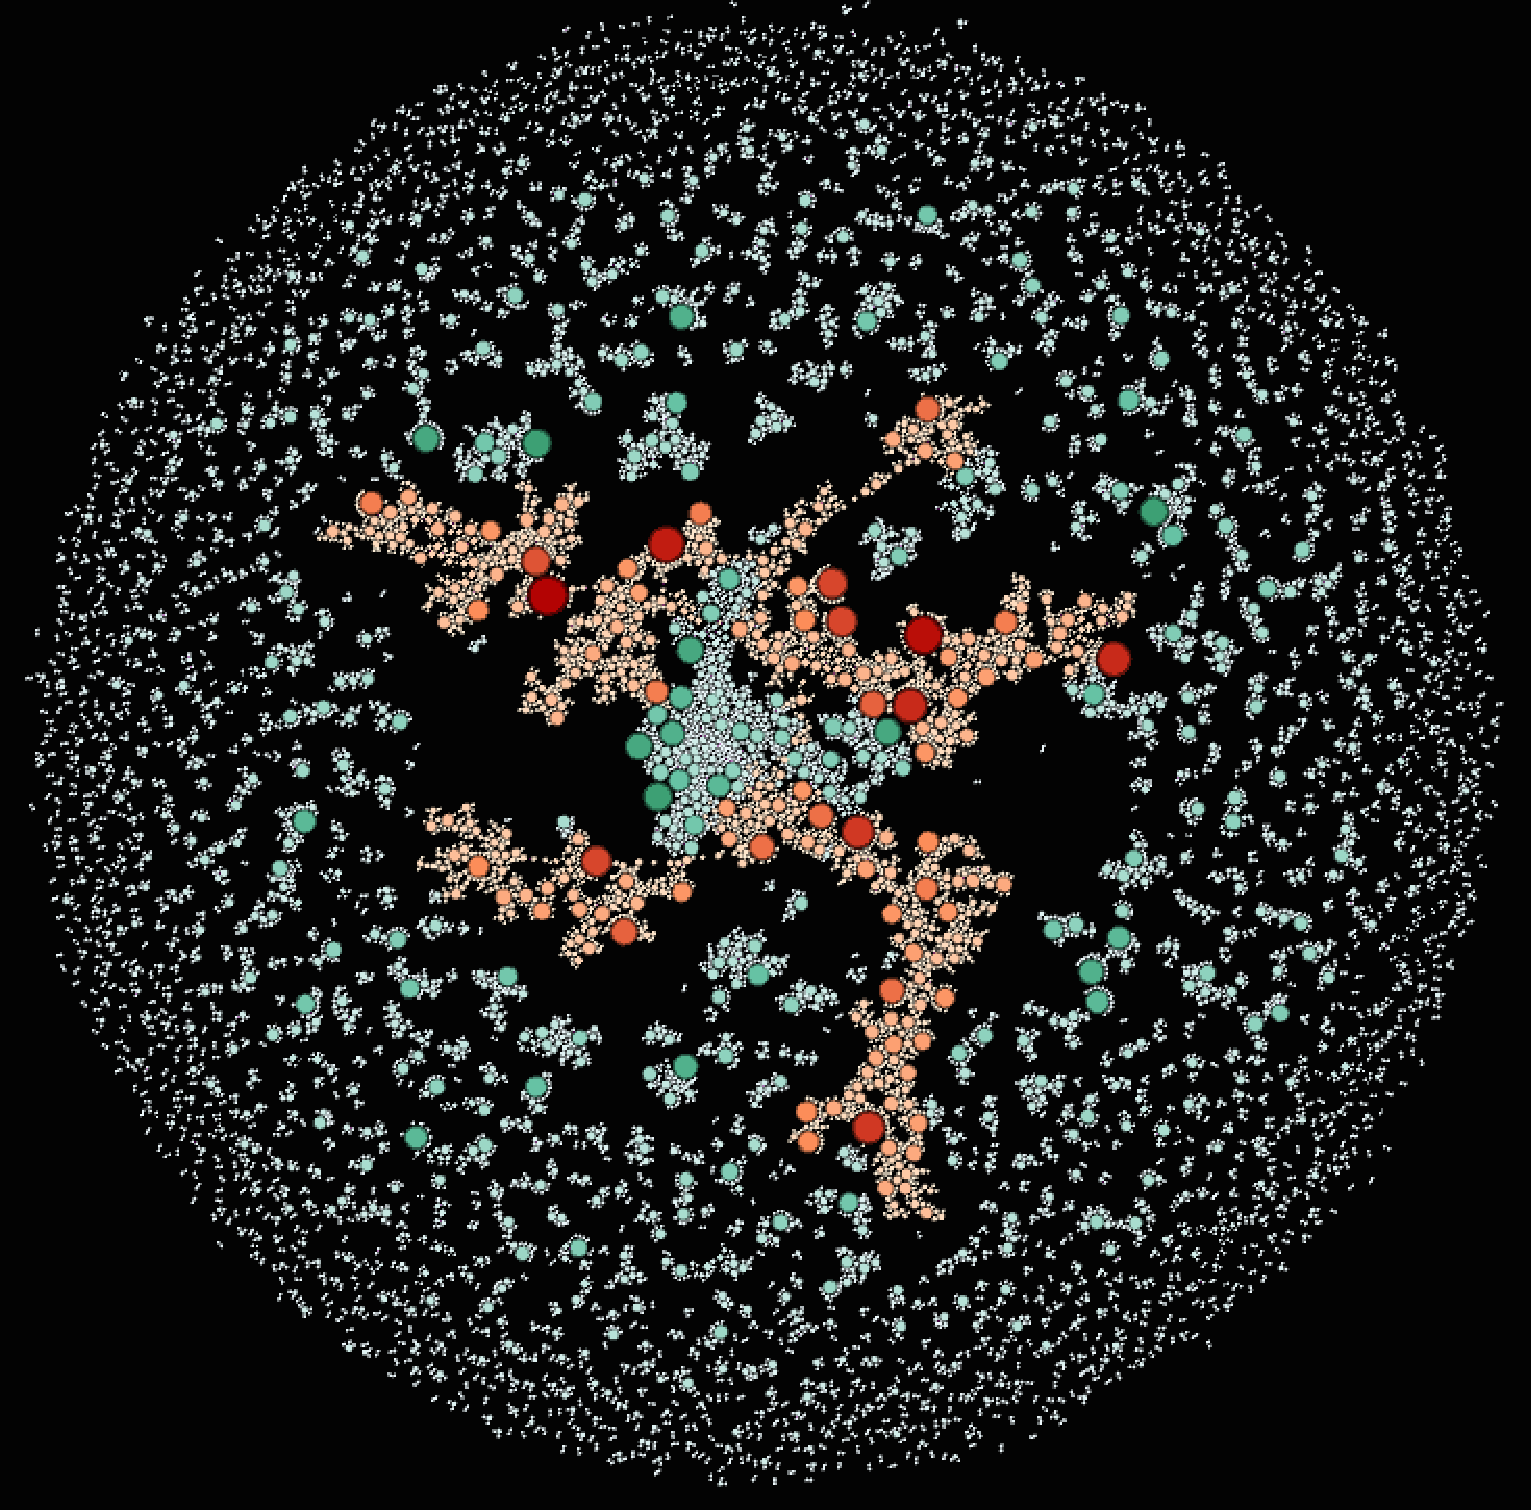
\includegraphics[width = 0.3\textwidth]{ProgramsImages/sexualNetworkNOLA}
	 \end{center}
	\caption{Heterosexual network for stochastic simulation of STD transmission.}.
	\label{netmodel}
\end{wrapfigure}
Public Health and Topical Medicine to develop a stochastic Monte Carlo Markov Chain agent-based model for the transmission of sexually transmitted diseases (STDs) in New Orleans \cite{azizi2018using}.  
The STIs spread through a dynamic heterosexual bipartite network of 20,000 nodes and include treatment, contact tracing, condom use, and partner notification. The network changes each day as people change their short-term and long-term partnerships.  
Since the partnership network and disease transmission is modeled as a stochastic process, multiple simulations with the same parameter values produce a multivariate  distribution of QOIs.  Each ensemble of runs can take hours on the Tulane Cypress 300+ TFlop supercomputer. 
We will use our adaptive sampling to help guide the optimization of different mitigation efforts for slowing the spread of STIs.  
In this example the mean-field MLS model will identify the underlying trends in the predictions, and the kriging Gaussian Process model will quantify the aleatory uncertainty created by the stochastic events.


%%%%%%%%%%%%%%%%%%%%%%%%%%%%%%%%%%%%%%%%%%%%%%%%%%%%%%%%%%%%%%%%%%%%%%%%%%%%%%%%%%%
\subsection{Software}  \label{sec:Software}
%%%%%%%%%%%%%%%%%%%%%%%%%%%%%%%%%%%%%%%%%%%%%%%%%%%%%%%%%%%%%%%%%%%%%%%%%%%%%%%%%%%
There is considerable interest in the computational mathematics, computer science, and engineering communities in developing and using software for the adaptive design and analysis of computer experiments.  Examples of existing packages are the MATLAB libraries UQLab \cite{UQLab2014}, SUMO\cite{SUMO2010}, ooDACE \cite{ooDACE2014} (a successor to DACE \cite{dace2002}), and CODES \cite{CODES2015}, and the Python libraries emukit \cite{emukit2019}, SMT \cite{SMT2019}, and pySOT \cite{pySOT2015}.  Many of these packages employ allow for trends and variation modeling via kriging, but not their not as flexible, as those we intend to develop.

Our algorithms will be implemented in libraries on open source repositories for use by the modeling community.  We will compare the performance of our algorithms with existing software using test cases in the literature and on the large applications described above.  We will also explore collaborations with the developers of software libraries whose interests overlap ours so that we can leverage each others' strengths.

%%%%%%%%%%%%%%%%%%%%%%%%%%%%%%%%%%%%%%%%%%%%%%%%%%%%%%%%%%%%%%%%%%%%%%%%%%%%%%%%%%%

\section{Broader Impact of our Proposed Research and Development Plan}

%%%%%%%%%%%%%%%%%%%%%%%%%%%%%%%%%%%%%%%%%%%%%%%%%%%%%%%%%%%%%%%%%%%%%%%%%%%%%%%%%%%
The PIs will collaborating with a number of junior scholars, including students at the high school through PhD level.  Because this project spans theory, algorithms, applications, and software, we will be able to mentor our junior scholars in the areas that they have particular interest or ability, while helping them to understand the spectrum of expertise required to solve these kinds of problems.  The PIs will also engage in giving tutorials and teaching courses that will include our new results.

%%%%%%%%%%%%%%%%%%%%%%%%%%%%%%%%%%%%%%%%%%%%%%%%%%%%
%\subsection{Contributions to Training, Mentoring and Other Human Resource Developments}
%%%%%%%%%%%%%%%%%%%%%%%%%%%%%%%%%%%%%%%%%%%%%%%%%%%%
FJH and JMH lead regular research group meetings at their respective instituions comprised of long-term and short-term student 
collaborators, visitors, the curious, and special guests.  Ongoing work in early or polished stages is shared.  Papers of other authors are presented.  Mentoring takes place during these meetings as well as individually.

%%%%%%%%%%%%%%%%%%%%%%%%%%%%%%%%%%%%%%%%%%%%%%%%%%%%
\paragraph*{Providing Research Experiences for Undergraduate and High School Students} 
%%%%%%%%%%%%%%%%%%%%%%%%%%%%%%%%%%%%%%%%%%%%%%%%%%%%
Our project will support two summer undergraduate students per year at Illinois Tech, or possibly at LANL. As in the past, we expect the NSF funds will serve as a catalyst for funds to 
support additional summer students. In choosing summer students we will make a deliberate effort to 
build 
a diverse research environment by targeting female and underrepresented minority students as well 
as students from less research-focused institutions (see Sect.~\ref{prevBIsect}). We will also 
welcome well-prepared high school students to join our research group.

%%%%%%%%%%%%%%%%%%%%%%%%%%%%%%%%%%%%%%%%%%%%%%%%%%%%
\paragraph*{Preparing Students for Academic Careers} 
%%%%%%%%%%%%%%%%%%%%%%%%%%%%%%%%%%%%%%%%%%%%%%%%%%%%
Mentoring is a multi-faceted and 
potentially long-term process continuing even after the mentee has moved on from Illinois Tech.  
Our PhD students gain experience in both research and mentoring the younger students in our 
research group.  We 
continue contact with many of our former students, in particular Yiou Li (female).  We will continue to help our students prepare for 
academic careers and continue mentoring them after they leave Illinois Tech.

%%%%%%%%%%%%%%%%%%%%%%%%%%%%%%%%%%%%%%%%%%%%%%%%%%%%
\paragraph*{Preparing Students for Industry Careers}
%%%%%%%%%%%%%%%%%%%%%%%%%%%%%%%%%%%%%%%%%%%%%%%%%%%%
We also help current students land 
competitive jobs in the business world. Our training in the areas of computation and software 
development gives our students the needed edge in comparison to other mathematics 
graduates. For example, LlAJR and XZ are working in the financial services industry and  LJ is 
working in marketing analytics.  All of them are developing and testing quantitatively sophisticated and computationally intensive models. 

%%%%%%%%%%%%%%%%%%%%%%%%%%%%%%%%%%%%%%%%%%%%%%%%%%%%
\paragraph*{Giving Tutorials and Invited Lectures}
%%%%%%%%%%%%%%%%%%%%%%%%%%%%%%%%%%%%%%%%%%%%%%%%%%%%
We will continue providing lectures to students at various stages in their careers, ranging from high school to graduate school. These encourage students to enter STEM and encourage STEM students 
to engage in research in general, and this research area in particular.


%%%%%%%%%%%%%%%%%%%%%%%%%%%%%%%%%%%%%%%%%%%%%%%%%%%%
\subsection{Contributions to Resources in Research, Education and the Broader Society} 
\label{BroaderTwoSec}
%%%%%%%%%%%%%%%%%%%%%%%%%%%%%%%%%%%%%%%%%%%%%%%%%%%%

The proposed research straddles mathematics, statistics, theoretical computer science, and 
application areas.  The PIs have complementary strengths that facilitate this interdisciplinary research.  YD has expertise in adaptive algorithms and software development.  FJH has expertise in adaptive algorithms, low discrepancy sampling, kernel-based methods, and tractability. JMH has expertise in modeling of large scale phenomena and algorithm development.  Our 
expertise provides both an obligation and an opportunity to interact with a number of diverse 
communities. We envision the following contributions:

%%%%%%%%%%%%%%%%%%%%%%%%%%%%%%%%%%%%%%%%%%%%%%%%%%%%
\paragraph*{Disseminating Research and Writing Survey Papers}
%%%%%%%%%%%%%%%%%%%%%%%%%%%%%%%%%%%%%%%%%%%%%%%%%%%%
The research supported by this grant will result in publications in peer-reviewed journals in applied mathematics, computer science, statistics, and science/engineering. These 
journals will include both those that emphasize theory and those that emphasize applications.  The PIs will continue their practice of writing tutorial, survey, and encyclopedia articles.  These will make our findings accessible to a wider audience.


%%%%%%%%%%%%%%%%%%%%%%%%%%%%%%%%%%%%%%%%%%%%%%%%%%%%
\paragraph*{Organizing and Presenting at Conferences}
%%%%%%%%%%%%%%%%%%%%%%%%%%%%%%%%%%%%%%%%%%%%%%%%%%%%
We and our students involved in this project will present our results at a variety of conferences and workshops.  These include: (i) specialized meetings focusing on approximation theory, complexity, 
experimental design, Monte Carlo methods, and probabilistic numerics; (ii) the national meetings of AMS, SIAM, and the 
statistical societies; and (iii) conferences devoted to application areas.  We are frequently invited to 
speak at such conferences, which will give our results a prominent hearing. We will also continue to 
organize specialized conferences or minisymposia within larger conferences.

%%%%%%%%%%%%%%%%%%%%%%%%%%%%%%%%%%%%%%%%%%%%%%%%%%%%
\paragraph*{Bridging Applied Mathematics and Statistics}
%%%%%%%%%%%%%%%%%%%%%%%%%%%%%%%%%%%%%%%%%%%%%%%%%%%%
This project touches on topics that are of interest to the statistics community: kriging, Monte Carlo methods, probabilistic numerics, and design of experiments.  We have and will continue to engage the statistics community 
by speaking a their conferences and departmental colloquia.

%%%%%%%%%%%%%%%%%%%%%%%%%%%%%%%%%%%%%%%%%%%%%%%%%%%%
\paragraph*{Establishing a New Paradigm for Adaptive Algorithms} 
%%%%%%%%%%%%%%%%%%%%%%%%%%%%%%%%%%%%%%%%%%%%%%%%%%%%
The idea of adaptive algorithms where the sampling scheme and the norm of the input function adapts to the output data is uncommon in the computational mathematics literature.  The derivation of theory for adaptive algorithms based on cones is also new.  These ideas have potential applications to to other numerical problems beyond those studied in the proposed research.  We will continue to promote these ideas among numerical analysts and computational complexity theorists.  The recent work by Kunsch, Novak, and Rudolf \cite{KunEtal19a} shows that the idea of cones is catching on.

%%%%%%%%%%%%%%%%%%%%%%%%%%%%%%%%%%%%%%%%%%%%%%%%%%%%
\paragraph*{Creating Software and Collaborating with Software Developers}
%%%%%%%%%%%%%%%%%%%%%%%%%%%%%%%%%%%%%%%%%%%%%%%%%%%%
Our algorithms will be implemented in freely available software on public repositories.  We will discuss with software developers whose packages have complementary capabilities how we might collaborate. We expect our new algorithms to be incorporated into widely used numerical packages, as was done for our algorithm in \cite{HonHic00a} by \MATLAB and \NAG.  The \MATLAB \GAIL library \citep{ChoEtal19a}, developed by FJH, YD, and collaborators contains univariate function approximation and minimization algorithms, as well as multivariate integration algorithms.  A project to a community based quasi-Monte Carlo Python library QMCPy, is underway with corporate sponsorship.  

%%%%%%%%%%%%%%%%%%%%%%%%%%%%%%%%%%%%%%%%%%%%%%%%%%%%
\section{Project Management and Collaboration}
%%%%%%%%%%%%%%%%%%%%%%%%%%%%%%%%%%%%%%%%%%%%%%%%%%%%
This research will be primarily conducted at Illinois Tech, Tulane U, and Los Alamos National Laboratory (LANL), where JMH has visiting scientist appointment.  FJH will lead the effort at Illinois Tech, and JMH will lead the effort at Tulane.  FJH and YD will focus on the theoretical analysis of the algorithms, including error bounds for the surrogate models.  They will also lead the exploration of the data-inferred reproducing/covariance kernels.  JMH will focus on the design of our novel algorithms, including the weighted least squares and the Bayesian bootstrap.  He will also lead the application of our new algorithms to the large-scale application problems.  

The PhD student will be based at Illinois Tech during the academic year under the direct supervision of FJH and YD.  The PhD student will work on part of the algorithmic developments, its theoretical analysis, and its implementation in freely available software.  During the summer, the PhD student will join JMH in Los Alamos and be involved with testing our algorithms on challenging application problems.  The undergraduate students will work either at Illinois Tech or at LANL during the summer exploring interesting bite-sized aspects of the algorithms and their performance.

Our research groups will meet regularly via video conference and in person a couple of times per year at one of our campuses or at conferences.


%%%%%%%%%%%%%%%%%%%%%%%%%%%%%%%%%%%%%%%%%%%%%%%%%%%%%%%%%%%%%%%%%%%%%%%%%%%%%%%%%%%
\section{Results of Previous NSF-Funded Research,
NSF-DMS-1522687\except{toc}{, \\ \emph{Stable, Efficient, Adaptive Algorithms for 
Approximation and Integration}, \\
\$270,000, August 2015 -- July 2018}
} \label{sec:Previous}
%%%%%%%%%%%%%%%%%%%%%%%%%%%%%%%%%%%%%%%%%%%%%%%%%%%%%%%%%%%%%%%%%%%%%%%%%%%%%%%%%%%

Gregory E.\ Fasshauer (GEF, co-PI) and FJH (PI) led this project, and Sou-Cheng Terrya Choi (SCTC) contributed as senior personnel.  Other major contributors were FJH's research students Yuhan Ding (YD, PhD 2015), Lan Jiang (LJ, PhD 2016), 
Llu\'is Antoni Jim\'enez Rugama (LlAJR, PhD 2016), Da Li (DL, MS 2016), Jiazhen Liu (JL, MS 2018), Jagadeeswaran Rathinavel (JR, 
PhD student), Xin Tong (XT, MS 2014, PhD student, University of Illinois at Chicago), Kan Zhang (KZ, PhD student), Yizhi Zhang (YZ, PhD 2018), and Xuan Zhou (XZ, PhD 2015).  Articles, theses,  
software, and preprints supported in 
part by this 
grant 
include 
\cite{ala_augmented_2017, 
	ChoEtal17a,
	ChoEtal17b,
	Din15a, 
	DinHic20a,
	GilEtal16a,
	Hic17a,
	HicJag18b,
	HicJim16a,
	HicEtal18a,
	HicEtal17a,
	HicKriWoz19a,
	RatHic19a,
	GilJim16b,
	JimHic16a,
	JohFasHic18a,
	Li16a,
	Liu17a,
	MarEtal18a,
	mccourt_stable_2017,
	MCCEtal19a,
	mishra_hybrid_2018,
	MisEtal19a,
	rashidinia_stable_2016,
	rashidinia_stable_2018,
	Zha18a,
	Zha17a,
	Zho15a,
	ZhoHic15a}.

%%%%%%%%%%%%%%%%%%%%%%%%%%%%%%%%%%%%%%%%%%%%%%%%%%%%%%%%%%%%%%%%%%%%%%%%%%%%%%%%%%%
\subsection{Intellectual Merit from Previous NSF Funding}
\label{previousmeritsubsec}
%%%%%%%%%%%%%%%%%%%%%%%%%%%%%%%%%%%%%%%%%%%%%%%%%%%%%%%%%%%%%%%%%%%%%%%%%%%%%%%%%%%

%%%%%%%%%%%%%%%%%%%%%%%%%%%%%%%%%%%%%%%%%%%%%%%%%%%%%%%%%%%%%%%%%%%%%%%%%%%%%%%%%%%
\paragraph*{Adaptive Algorithms for Univariate Problems} \label{sec:localadpat}
%%%%%%%%%%%%%%%%%%%%%%%%%%%%%%%%%%%%%%%%%%%%%%%%%%%%%%%%%%%%%%%%%%%%%%%%%%%%%%%%%%%
\begin{wrapfigure}{r}{0.4\textwidth}
	\centering
	\vspace{-1ex}
	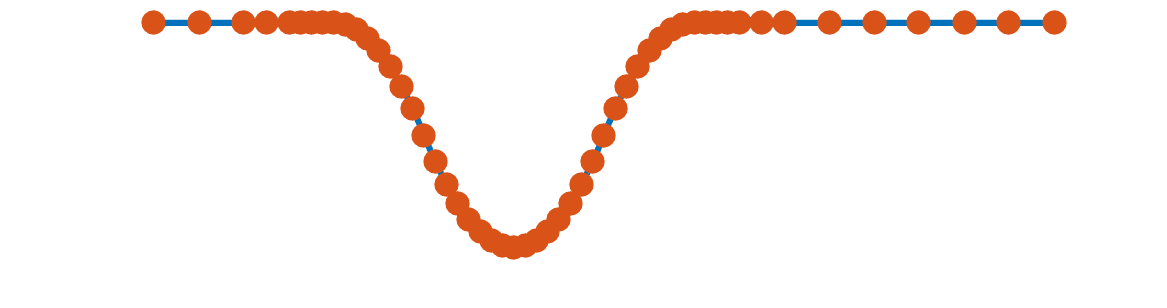
\includegraphics[width = 0.4\textwidth]{ProgramsImages/sampling-funappxg.png}
	\\
	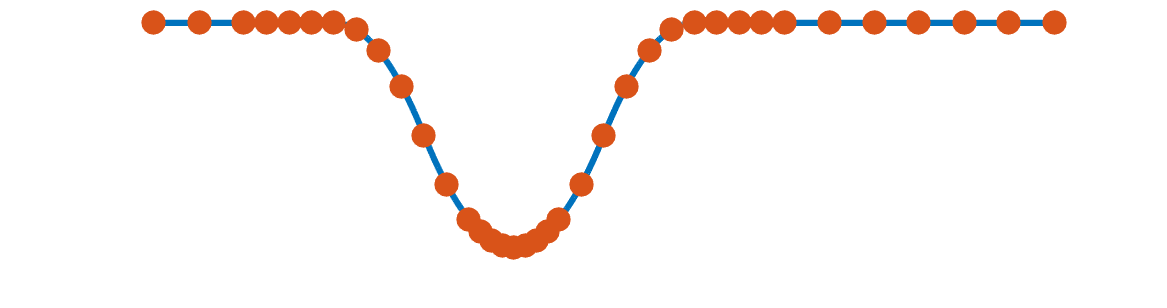
\includegraphics[width = 0.4\textwidth]{ProgramsImages/sampling-funming.png}

	\vspace{-2ex}
	\caption{The function data ({\color{MATLABOrange}$\bullet$}) for the locally adaptive 
	function approximation (top) and minimization (bottom) algorithms in \cite{ChoEtal17a}.  Sampling is denser where $\abs{f''}$ is larger.  For miminization it is also denser where the function values are smaller. \label{localadaptfig}}
\end{wrapfigure}

FJH, STSC, YD, XT, YZ and collaborators developed several adaptive algorithms for univariate integration, function approximation, and optimization \cite{ChoEtal17a,HicEtal14b,  Din15a, Ton14a, Zha18a}.  Most of these algorithms are \emph{globally adaptive}---the sampling density is constant, but the number of data sites is chosen adaptively to meet the error tolerance.

However, the function approximation and integration algorithms constructed by FJH, SCTC, YD, and XT in \cite{ChoEtal17a} are \emph{locally adaptive}, meaning that the sampling density is non-uniform and influenced by the function data.  Qualitatively, the cone of functions for which these algorithms are guaranteed to succeed consists of functions where the maximum of the second derivative in a sub-interval is not drastically smaller than the larger of it's minimum value to the immediate left or right.  For function approximation, the adaptive sample is denser where $\abs{f''}$ is larger, as shown in Fig.\ \ref{localadaptfig}.  This locally adaptive function approximation algorithm has a computational cost of $\Order\left(\sqrt{\norm[1/2]{f''}/\varepsilon} \right)$, where $\varepsilon$ is the error tolerance, and is essentially optimal.  An intriguing aspect is the appearance of the $1/2$-quasinorm $\norm[1/2]{f''}$, which may be much smaller than 
$\norm[\infty]{f''}$ for peaky functions.



%%%%%%%%%%%%%%%%%%%%%%%%%%%%%%%%%%%%%%%%%%%%%%%%%%%%%%%%%%%%%%%%%%%%%%%%%%%%%%%%%%%
\paragraph*[QMCsec]{Globally Adaptive Cubature Based on Space-Filling Designs} \hypertarget{QMClink}{}
\label{sec:QMC}
%%%%%%%%%%%%%%%%%%%%%%%%%%%%%%%%%%%%%%%%%%%%%%%%%%%%%%%%%%%%%%%%%%%%%%%%%%%%%%%%%%%

FJH, LlAJR, DL, and JR developed globally adaptive algorithms for approximating $d$-dimensional integrals,  $\int_{[0,1]^d} f(\bx) \, \dif \bx$, based on space-filling designs \cite{HicJim16a,HicEtal17a,JimHic16a}.  Two common space-filling or low discrepancy designs are integration lattice nodes and digital sequences \cite{DicEtal14a} (see   Fig.\ \ref{PtsFig}). 

The error bounds underlying the adaptive cubatures developed by FJH, LlAJR, DL are based on the Fourier coefficients of the sampled function values on these space-filling designs.  The Fourier  \{complex exponential/Walsh functions\} bases are chosen to match the \{lattices/ digital sequences\}  designs, which makes the cubature error bounds possible.  The globally adaptive cubatures increase $n$ by powers of two until the error bounds are no greater than the error tolerance, $\varepsilon$.  The cones, $\calc$, of integrands for which these adaptive cubatures are guaranteed are those for which  the Fourier coefficients decay steadily, but not necessarily monotonically, in magnitude.

FJH and JR  assumed that the integrand is an instance of a Gaussian process with constant mean $m$, and covariance kernel, $K:[0,1]^d \times [0,1]^d \to \reals$.  The same space-filling designs are used as are pictured in Fig.\ \ref{PtsFig}.  A $99\%$ credible interval for the integral is constructed.  The sample size, $n$, is increased until the half-width is no greater than the error tolerance, $\varepsilon$, the algorithm terminates.  The hyper-parameters, $m$ and the parameters defining the covariance kernel, $K$, may be treated by empirical Bayes (maximum likelihood estimation), full Bayes, and/or cross-validation \cite{RatHic19a}. The major contribution of FJH and JR is to speed up the computational cost required by this Bayesian cubature.  Bayesian cubature requires operations
involving the Gram matrix $\mK$ defined in \eqref{appxExOne}, and ordinarily these operations  have a cost of
$\Order(n^3)$.  FJH and JR chose covariance kernels, $K$, which matched the space-filling designs and reduced the computational cost to $\Order(n 
\log(n))$, making Bayesian cubature practical.

%%%%%%%%%%%%%%%%%%%%%%%%%%%%%%%%%%%%%%%%%%%%%%%%%%%%%%%%%%%%%%%%%%%%%%%%%%%%%%%%%%%
\paragraph*{Multivariate Function Approximation} \label{sec:PrevFunAppx}
%%%%%%%%%%%%%%%%%%%%%%%%%%%%%%%%%%%%%%%%%%%%%%%%%%%%%%%%%%%%%%%%%%%%%%%%%%%%%%%%%%%

FJH, YD, and LlAJR and collaborators investigated the function approximation problems for Banach spaces, $\calf$, defined by general series representations \cite{DinHic20a,DinEtal20a}.  For example, the bases can be general multivariate polynomials.  Three different definitions of cone, $\calc$, of functions were defined, all describing a reasonable behavior of the series coefficients.  Adaptive function approximation algorithms were constructed for these three cones shown to be essentially optimal.  The shortcoming of this research is that the algorithms use series coefficients as data rather than function values. 


%%%%%%%%%%%%%%%%%%%%%%%%%%%%%%%%%%%%%%%%%%%%%%%%%%%%%%%%%%%%%%%%%%%%%%%%%%%%%%%%%%%
\subsection{Broader Impacts from Previous NSF Funding} \label{prevBIsect}
%%%%%%%%%%%%%%%%%%%%%%%%%%%%%%%%%%%%%%%%%%%%%%%%%%%%%%%%%%%%%%%%%%%%%%%%%%%%%%%%%%%

\paragraph*{Publications, Conference Participation, Conference Organization, and Leadership} Publications by GEF, FJH,  SCTC, students, and collaborators are listed at the beginning of this section.  We have spoken at many applied mathematics, statistics, 
and computational science conferences and given colloquium/seminar talks to mathematics and 
statistics departments.  FJH co-organized the 
2016 Spring Research 
Conference, a long-running annual industrial statistics conference.   FJH gave an invited tutorial
at MCQMC 2016
\cite{Hic17a}, a biennial conference for which he serves on the steering committee.  FJH 
was a program leader for the SAMSI 2017--18 Quasi-Monte Carlo (QMC) Program.   FJH received the 2016 Joseph F.\ Traub Prize for Achievement in Information-Based Complexity. In recognition of his research leadership, FJH was appointed the director of Illinois Tech's new Center for Interdisciplinary 
Scientific Computation in 2017.  In 2018, FJH was appointed Vice Provost for Research.
	
\paragraph*{\GAIL Software} The results of this research have been implemented in 
\GAIL, our open source \MATLAB library hosted on
Github. This software 
has been implemented with input parsing, input validation, unit tests, inline documentation, and 
demonstrations.  \GAIL makes it easier for practitioners to try our new adaptive algorithms.  SCTC has been key in this effort.  \GAIL has been used in the yearly graduate course in Monte Carlo methods taught by FJH and YD.  
%With the help of students, we are starting to port GAIL to Python and \Rlang.

\paragraph*{Boosting the STEM Workforce.} GEF, FJH, and SCTC mentored a number of 
research students associated with this project.  Female students mentored include YD, LJ, JL, XT, and Xiaoyang Zhao (MS 2017).   GEF, FJH,  and SCTC have mentored many undergraduate students including more than a dozen 
Brazilian Science Mobility Program students in the summers of 2015 and 2016, plus eight other students (two female) from Illinois Tech, Biola U, U Minnesota, Macalester U, NUS, Colorado School of Mines.  All but one have enrolled in graduate programs.   As part of our team, all of
these students have learned how to conduct theoretical and/or practical computational mathematics research.


\newpage
\clearpage
%\pagenumbering{arabic}
\setcounter{page}{1}
%\renewcommand{\thepage}{D-\arabic{page}}

\bibliographystyle{spbasic.bst}


{\renewcommand\addcontentsline[3]{} 
\renewcommand{\refname}{{\Large\textbf{References Cited}}}                   %%
\renewcommand{\bibliofont}{\normalsize}

\bibliography{DoE_MH,FJH23,FJHown23,yuhan}}
\end{document}
